\documentclass[10pt,fleqn]{article} % Default font size and left-justified equations
\usepackage[%
    pdftitle={Modélisation systèmes multiphysiques : Modélisation linéaire et non linéaire},
    pdfauthor={Xavier Pessoles}]{hyperref}
    
%%%%%%%%%%%%%%%%%%%%%%%%%%%%%%%%%%%%%%%%%
% Original author:
% Mathias Legrand (legrand.mathias@gmail.com) with modifications by:
% Vel (vel@latextemplates.com)
% License:
% CC BY-NC-SA 3.0 (http://creativecommons.org/licenses/by-nc-sa/3.0/)
%%%%%%%%%%%%%%%%%%%%%%%%%%%%%%%%%%%%%%%%%

%----------------------------------------------------------------------------------------
%	VARIOUS REQUIRED PACKAGES AND CONFIGURATIONS
%----------------------------------------------------------------------------------------

\usepackage[top=2.5cm,bottom=2cm,left=2cm,right=2cm,headsep=40pt,a4paper]{geometry} % Page margins

\usepackage{graphicx} % Required for including pictures
\graphicspath{{images/}} % Specifies the directory where pictures are stored

\usepackage{lipsum} % Inserts dummy text

\usepackage{tikz} % Required for drawing custom shapes

\usepackage[french]{babel} % English language/hyphenation
\frenchbsetup{StandardLists=true} % Pour éviter la collision babel enumitem pour les listes

\usepackage{enumitem} % Customize lists
\setlist{nolistsep} % Reduce spacing between bullet points and numbered lists

\usepackage{booktabs} % Required for nicer horizontal rules in tables

\usepackage{xcolor} % Required for specifying colors by name
%\definecolor{ocre}{RGB}{243,102,25} % Define the orange color used for highlighting throughout the book
 \definecolor{ocre}{RGB}{49,133,156} % Couleur ''bleue''
\definecolor{violetf}{RGB}{112,48,160} % Couleur ''violet''
\usepackage{enumitem}
\usepackage{pifont} % Pour les dinglist
\usepackage{multicol}
\usepackage{array} % Centrage vertical dans les tableaux

%----------------------------------------------------------------------------------------
%	FONTS
%----------------------------------------------------------------------------------------

\usepackage{avant} % Use the Avantgarde font for headings
%\usepackage{times} % Use the Times font for headings
%\usepackage{mathptmx} % Use the Adobe Times Roman as the default text font together with math symbols from the Sym­bol, Chancery and Com­puter Modern fonts
\usepackage[adobe-utopia]{mathdesign}
\usepackage{microtype} % Slightly tweak font spacing for aesthetics
\usepackage[utf8]{inputenc} % Required for including letters with accents
\usepackage[T1]{fontenc} % Use 8-bit encoding that has 256 glyphs

%----------------------------------------------------------------------------------------
%	BIBLIOGRAPHY AND INDEX
%----------------------------------------------------------------------------------------

\usepackage[style=alphabetic,citestyle=numeric,sorting=nyt,sortcites=true,autopunct=true,babel=hyphen,hyperref=true,abbreviate=false,backref=true,backend=biber]{biblatex}
\addbibresource{bibliography.bib} % BibTeX bibliography file
\defbibheading{bibempty}{}

\usepackage{calc} % For simpler calculation - used for spacing the index letter headings correctly
\usepackage{makeidx} % Required to make an index
\makeindex % Tells LaTeX to create the files required for indexing

%----------------------------------------------------------------------------------------
%	MAIN TABLE OF CONTENTS
%----------------------------------------------------------------------------------------

\usepackage{titletoc} % Required for manipulating the table of contents

\setcounter{tocdepth}{2}     % Dans la table des matieres
\setcounter{secnumdepth}{2}

\contentsmargin{0cm} % Removes the default margin

% Part text styling
\titlecontents{part}[0cm]
{\addvspace{20pt}\centering\large\bfseries}
{}
{}
{}

% Chapter text styling
\titlecontents{chapter}[1.25cm] % Indentation
{\addvspace{12pt}\large\sffamily\bfseries} % Spacing and font options for chapters
{\color{ocre!60}\contentslabel[\Large\thecontentslabel]{1.25cm}\color{ocre}} % Chapter number
{\color{ocre}}  
{\color{ocre!60}\normalsize\;\titlerule*[.5pc]{.}\;\thecontentspage} % Page number

% Section text styling
\titlecontents{section}[1.25cm] % Indentation
{\addvspace{3pt}\sffamily\bfseries} % Spacing and font options for sections
{\color{ocre!60}\contentslabel[\thecontentslabel]{1.25cm} \color{ocre}} % Section number
{\color{ocre}}
{\hfill\color{ocre!60}\thecontentspage} % Page number
[]

% Subsection text styling
\titlecontents{subsection}[1.25cm] % Indentation
{\addvspace{1pt}\sffamily\small} % Spacing and font options for subsections
{\contentslabel[\thecontentslabel]{1.25cm}} % Subsection number
{}
{\ \titlerule*[.5pc]{.}\;\thecontentspage} % Page number
[]


% Subsection text styling
\titlecontents{subsubsection}[1.25cm] % Indentation
{\addvspace{1pt}\sffamily\small} % Spacing and font options for subsections
{\contentslabel[\thecontentslabel]{1.25cm}} % Subsection number
{}
{\ \titlerule*[.5pc]{.}\;\thecontentspage} % Page number
[]

% List of figures
\titlecontents{figure}[0em]
{\addvspace{-5pt}\sffamily}
{\thecontentslabel\hspace*{1em}}
{}
{\ \titlerule*[.5pc]{.}\;\thecontentspage}
[]

% List of tables
\titlecontents{table}[0em]
{\addvspace{-5pt}\sffamily}
{\thecontentslabel\hspace*{1em}}
{}
{\ \titlerule*[.5pc]{.}\;\thecontentspage}
[]

%----------------------------------------------------------------------------------------
%	MINI TABLE OF CONTENTS IN PART HEADS
%----------------------------------------------------------------------------------------

% Chapter text styling
\titlecontents{lchapter}[0em] % Indenting
{\addvspace{15pt}\large\sffamily\bfseries} % Spacing and font options for chapters
{\color{ocre}\contentslabel[\Large\thecontentslabel]{1.25cm}\color{ocre}} % Chapter number
{}  
{\color{ocre}\normalsize\sffamily\bfseries\;\titlerule*[.5pc]{.}\;\thecontentspage} % Page number

% Section text styling
\titlecontents{lsection}[0em] % Indenting
{\sffamily\small} % Spacing and font options for sections
{\contentslabel[\thecontentslabel]{1.25cm}} % Section number
{}
{}

% Subsection text styling
\titlecontents{lsubsection}[.5em] % Indentation
{\normalfont\footnotesize\sffamily} % Font settings
{}
{}
{}

%----------------------------------------------------------------------------------------
%	PAGE HEADERS
%----------------------------------------------------------------------------------------

\usepackage{fancyhdr} % Required for header and footer configuration



\pagestyle{fancy}
 \renewcommand{\headrulewidth}{0pt}
 \fancyhead{}
 \fancyhead[L]{%
 \noindent\begin{minipage}[c]{2.6cm}%
 
\includegraphics[width=2cm]{png/logo_upsti.png}%
 \end{minipage}}

\fancyhead[C]{\rule{8cm}{.5pt}}

 \fancyhead[R]{%
 \noindent\begin{minipage}[c]{3cm}
 \begin{flushright}
 \footnotesize{\textit{\textsf{\xxtete}}}%
 \end{flushright}
 \end{minipage}
}


\fancyfoot[C]{\rule{12cm}{.5pt}}
\renewcommand{\footrulewidth}{0.2pt}
\fancyfoot[C]{\footnotesize{\bfseries \thepage}}
\fancyfoot[L]{ 
\begin{minipage}[c]{.4\linewidth}
\noindent\footnotesize{{\xxauteur}}
\end{minipage}}


\fancyfoot[R]{\footnotesize{\xxpied}
\ifthenelse{\isodd{\value{page}}}{
\begin{tikzpicture}[overlay]
\node[shape=rectangle, 
      rounded corners = .25 cm,
	  draw= ocre,
	  line width=2pt, 
	  fill = ocre!10,
	  minimum width  = 2.5cm,
	  minimum height = 3cm,] at (\xxposongletx,\xxposonglety) {};
\node at (\xxposonglettext,\xxposonglety) {\rotatebox{90}{\textbf{\large\color{ocre}{\xxonglet}}}};
%{};
\end{tikzpicture}}{}
}
%
%
%
% Removes the header from odd empty pages at the end of chapters
\makeatletter
\renewcommand{\cleardoublepage}{
\clearpage\ifodd\c@page\else
\hbox{}
\vspace*{\fill}
\thispagestyle{empty}
\newpage
\fi}

\fancypagestyle{plain}{%
\fancyhf{} % vide l’en-tête et le pied~de~page.
%\fancyfoot[C]{\bfseries \thepage} % numéro de la page en cours en gras
% et centré en pied~de~page.
\fancyfoot[R]{\footnotesize{\xxpied}}
\fancyfoot[C]{\rule{12cm}{.5pt}}
\renewcommand{\footrulewidth}{0.2pt}
\fancyfoot[C]{\footnotesize{\bfseries \thepage}}
\fancyfoot[L]{ 
\begin{minipage}[c]{.4\linewidth}
\noindent\footnotesize{{\xxauteur}}
\end{minipage}}}



%----------------------------------------------------------------------------------------
%	THEOREM STYLES
%----------------------------------------------------------------------------------------

% Conflit avec la police adobe
%\usepackage{amsmath,amsfonts,amssymb,amsthm} % For math equations, theorems, symbols, etc
\usepackage{amsmath,amsthm}

\newcommand{\intoo}[2]{\mathopen{]}#1\,;#2\mathclose{[}}
\newcommand{\ud}{\mathop{\mathrm{{}d}}\mathopen{}}
\newcommand{\intff}[2]{\mathopen{[}#1\,;#2\mathclose{]}}
%\newtheorem{notation}{Notation}[chapter]
\newtheorem{notation}{Notation}[section]

% Boxed/framed environments
\newtheoremstyle{ocrenumbox}% % Theorem style name
{0pt}% Space above
{0pt}% Space below
{\normalfont}% % Body font
{}% Indent amount
{\small\bf\sffamily\color{ocre}}% % Theorem head font
{\;}% Punctuation after theorem head
{0.25em}% Space after theorem head
{\small\sffamily\color{ocre}\thmname{#1}\nobreakspace\thmnumber%{\@ifnotempty{#1}{}\@upn{#2}}% Theorem text (e.g. Theorem 2.1)
\thmnote{\nobreakspace\the\thm@notefont\sffamily\bfseries\color{black}---\nobreakspace#3.}} % Optional theorem note
\renewcommand{\qedsymbol}{$\blacksquare$}% Optional qed square


% Boite pour les corriges
\newtheoremstyle{correctionbox}% % Theorem style name
{0pt}% Space above
{0pt}% Space below
{\normalfont}% % Body font
{}% Indent amount
{\small\bf\sffamily\color{violet}}% % Theorem head font
{\;}% Punctuation after theorem head
{0.25em}% Space after theorem head
{\small\sffamily\color{ocre}\thmname{#1}\nobreakspace\thmnumber%{\@ifnotempty{#1}{}\@upn{#2}}% Theorem text (e.g. Theorem 2.1)
\thmnote{\nobreakspace\the\thm@notefont\sffamily\bfseries\color{black}---\nobreakspace#3.}} % Optional theorem note
\renewcommand{\qedsymbol}{$\blacksquare$}% Optional qed square



\newtheoremstyle{blacknumex}% Theorem style name
{5pt}% Space above
{5pt}% Space below
{\normalfont}% Body font
{} % Indent amount
{\small\bf\sffamily}% Theorem head font
{\;}% Punctuation after theorem head
{0.25em}% Space after theorem head
{\small\sffamily{\tiny\ensuremath{\blacksquare}}\nobreakspace\thmname{#1}\nobreakspace\thmnumber%{\@ifnotempty{#1}{}\@upn{#2}}% Theorem text (e.g. Theorem 2.1)
\thmnote{\nobreakspace\the\thm@notefont\sffamily\bfseries---\nobreakspace#3.}}% Optional theorem note

\newtheoremstyle{blacknumbox} % Theorem style name
{0pt}% Space above
{0pt}% Space below
{\normalfont}% Body font
{}% Indent amount
{\small\bf\sffamily}% Theorem head font
{\;}% Punctuation after theorem head
{0.25em}% Space after theorem head
{\small\sffamily\thmname{#1}\nobreakspace 
\thmnote{\nobreakspace\the\thm@notefont\sffamily\bfseries---\nobreakspace#3.}}% Optional theorem note

% Non-boxed/non-framed environments
\newtheoremstyle{ocrenum}% % Theorem style name
{5pt}% Space above
{5pt}% Space below
{\normalfont}% % Body font
{}% Indent amount
{\small\bf\sffamily\color{ocre}}% % Theorem head font
{\;}% Punctuation after theorem head
{0.25em}% Space after theorem head
{\small\sffamily\color{ocre}\thmname{#1}\nobreakspace%\thmnumber{\@ifnotempty{#1}{}\@upn{#2}}% Theorem text (e.g. Theorem 2.1)
\thmnote{\nobreakspace\the\thm@notefont\sffamily\bfseries\color{black}---\nobreakspace#3.}} % Optional theorem note
\renewcommand{\qedsymbol}{$\blacksquare$}% Optional qed square
\makeatother

% Environnement pour les titres de parties
\newtheoremstyle{partiebox} 
{0pt}% Space above
{0pt}% Space below
{\normalfont}% Body font
{}% Indent amount
{\small\bf\sffamily}% Theorem head font
{\;}% Punctuation after theorem head
{0.25em}% Space after theorem head




% Defines the theorem text style for each type of theorem to one of the three styles above
\newcounter{dummy} 
\numberwithin{dummy}{section}
\theoremstyle{ocrenumbox}
%\newtheorem{theoremeT}[dummy]{Théorème}
\newtheorem{theoremeT}[dummy]{Théorème}
\newtheorem{resultatT}[dummy]{Résultat}
\newtheorem{savoirT}[dummy]{Savoir}
\newtheorem{methodeT}[dummy]{Méthode}
\newtheorem{objectifT}[dummy]{Objectif}
%\newtheorem{problem}{Problem}[chapter]
\newtheorem{problem}{Problem}[section]
%\newtheorem{exerciseT}{Exercise}[chapter]
\newtheorem{exerciseT}{Exercice}[section]

\theoremstyle{blacknumex}
%\newtheorem{exampleT}{Example}[chapter]
\newtheorem{exempleT}{Exemple}[section]
\newtheorem{termT}{Terminal\\}[section]
\newtheorem{pyT}{Python\\}[section]
\newtheorem{sciT}{Scilab\\}[section]
\newtheorem{pseudoT}{Pseudo Code\\}[section]
\newtheorem{sqlT}{SQL\\}[section]

\theoremstyle{blacknumbox}
%\newtheorem{vocabulary}{Vocabulary}[chapter]
\newtheorem{vocabulary}{Vocabulaire}[section]
%\newtheorem{definitionT}{Definition}[section]
\newtheorem{definitionT}{Définition}[section]
\newtheorem{rappelT}{Rappel}[section]
\newtheorem{demoT}{Démonstration}[section]
\newtheorem{corollaryT}[dummy]{Corollaire}
\newtheorem{hypoT}{Hypothèse(s)}

\theoremstyle{ocrenum}
\newtheorem{proposition}[dummy]{Proposition}

\theoremstyle{partiebox}
\newtheorem{titrepartieT}[]{}
\newtheorem{titrechapitreT}[]{}

\theoremstyle{correctionbox}
\newtheorem{correctionT}[dummy]{\color{violet}{Correction}}

%----------------------------------------------------------------------------------------
%	DEFINITION OF COLORED BOXES
%----------------------------------------------------------------------------------------

\RequirePackage[framemethod=tikz]{mdframed} % Required for creating the theorem, definition, exercise and corollary boxes

% Theorem box
\newmdenv[skipabove=7pt,
skipbelow=7pt,
backgroundcolor=ocre!10,
linecolor=ocre,
innerleftmargin=5pt,
innerrightmargin=5pt,
innertopmargin=5pt,
leftmargin=0cm,
rightmargin=0cm,
innerbottommargin=5pt]{tBox}


% Correction
\newmdenv[skipabove=7pt,
skipbelow=7pt,
backgroundcolor=violet!10,
linecolor=violet,
innerleftmargin=5pt,
innerrightmargin=5pt,
innertopmargin=5pt,
leftmargin=0cm,
rightmargin=0cm,
innerbottommargin=5pt]{coBox}


% Exercise box	  
\newmdenv[skipabove=7pt,
skipbelow=7pt,
rightline=false,
leftline=true,
topline=false,
bottomline=false,
backgroundcolor=ocre!10,
linecolor=ocre,
innerleftmargin=5pt,
innerrightmargin=5pt,
innertopmargin=5pt,
innerbottommargin=5pt,
leftmargin=0cm,
rightmargin=0cm,
linewidth=4pt]{eBox}	

% Definition box
\newmdenv[skipabove=7pt,
skipbelow=7pt,
rightline=false,
leftline=true,
topline=false,
bottomline=false,
backgroundcolor=ocre!10,
linecolor=ocre,
innerleftmargin=5pt,
innerrightmargin=5pt,
innertopmargin=0pt,
leftmargin=0cm,
rightmargin=0cm,
linewidth=4pt,
innerbottommargin=0pt]{dBox}	

% Demonstration box
\newmdenv[skipabove=7pt,
skipbelow=7pt,
rightline=false,
leftline=true,
topline=false,
bottomline=false,
%backgroundcolor=ocre!10,
linecolor=ocre,
innerleftmargin=5pt,
innerrightmargin=5pt,
innertopmargin=0pt,
leftmargin=0cm,
rightmargin=0cm,
linewidth=4pt,
innerbottommargin=0pt]{demoBox}	

% Corollary box
\newmdenv[skipabove=7pt,
skipbelow=7pt,
rightline=false,
leftline=true,
topline=false,
bottomline=false,
linecolor=gray,
backgroundcolor=black!5,
innerleftmargin=5pt,
innerrightmargin=5pt,
innertopmargin=5pt,
leftmargin=0cm,
rightmargin=0cm,
linewidth=4pt,
innerbottommargin=5pt]{cBox}


% Hypothèses
\newmdenv[skipabove=7pt,
skipbelow=7pt,
rightline=false,
leftline=true,
topline=false,
bottomline=false,
linecolor=gray,
backgroundcolor=black!5,
innerleftmargin=5pt,
innerrightmargin=5pt,
innertopmargin=5pt,
leftmargin=0cm,
rightmargin=0cm,
linewidth=4pt,
innerbottommargin=5pt]{hyBox}


% Boite pour le titre de la partie (pBox)
\newmdenv[skipabove=7pt,
skipbelow=7pt,
rightline=true,
leftline=false,
topline=false,
bottomline=false,
linecolor=ocre,
backgroundcolor=none,
innerleftmargin=5pt,
innerrightmargin=5pt,
innertopmargin=5pt,
leftmargin=0cm,
rightmargin=0cm,
linewidth=4pt,
innerbottommargin=5pt]{pBox}

% Boite pour le titre du chapitre (chBox)
\newmdenv[skipabove=7pt,
skipbelow=7pt,
rightline=false,
leftline=true,
topline=false,
bottomline=false,
linecolor=ocre,
%backgroundcolor=black!5,
innerleftmargin=5pt,
innerrightmargin=5pt,
innertopmargin=5pt,
leftmargin=0cm,
rightmargin=0cm,
linewidth=4pt,
innerbottommargin=5pt]{chBox}


% Boite pour les exemples
\newmdenv[skipabove=7pt,
skipbelow=7pt,
rightline=false,
leftline=true,
topline=false,
bottomline=false,
linecolor=gray,
backgroundcolor=white,
innerleftmargin=5pt,
innerrightmargin=5pt,
innertopmargin=5pt,
leftmargin=0cm,
rightmargin=0cm,
linewidth=4pt,
innerbottommargin=5pt]{exBox}

% Boite pour le terminal
\newmdenv[skipabove=7pt,
skipbelow=7pt,
rightline=false,
leftline=true,
topline=false,
bottomline=false,
linecolor=gray,
backgroundcolor=white,
innerleftmargin=5pt,
innerrightmargin=5pt,
innertopmargin=5pt,
leftmargin=0cm,
rightmargin=0cm,
linewidth=4pt,
innerbottommargin=5pt]{termBox}


% Boite pour Python
\newmdenv[skipabove=7pt,
skipbelow=7pt,
rightline=false,
leftline=true,
topline=false,
bottomline=false,
linecolor=gray,
backgroundcolor=white,
innerleftmargin=5pt,
innerrightmargin=5pt,
innertopmargin=0pt,
leftmargin=0cm,
rightmargin=0cm,
linewidth=4pt,
innerbottommargin=5pt]{pyBox}

% Boite pour scilab
\newmdenv[skipabove=7pt,
skipbelow=7pt,
rightline=false,
leftline=true,
topline=false,
bottomline=false,
linecolor=gray,
backgroundcolor=white,
innerleftmargin=5pt,
innerrightmargin=5pt,
innertopmargin=5pt,
leftmargin=0cm,
rightmargin=0cm,
linewidth=4pt,
innerbottommargin=5pt]{sciBox}


% Boite pour pseudo
\newmdenv[skipabove=7pt,
skipbelow=7pt,
rightline=false,
leftline=true,
topline=false,
bottomline=false,
linecolor=gray,
backgroundcolor=white,
innerleftmargin=5pt,
innerrightmargin=5pt,
innertopmargin=5pt,
leftmargin=0cm,
rightmargin=0cm,
linewidth=4pt,
innerbottommargin=5pt]{pseudoBox}

% Boite pour pseudo
\newmdenv[skipabove=7pt,
skipbelow=7pt,
rightline=false,
leftline=true,
topline=false,
bottomline=false,
linecolor=gray,
backgroundcolor=white,
innerleftmargin=5pt,
innerrightmargin=5pt,
innertopmargin=5pt,
leftmargin=0cm,
rightmargin=0cm,
linewidth=4pt,
innerbottommargin=5pt]{sqlBox}


% Creates an environment for each type of theorem and assigns it a theorem text style from the "Theorem Styles" section above and a colored box from above
\newenvironment{theorem}{\begin{tBox}\begin{theoremeT}}{\end{theoremeT}\end{tBox}}
\newenvironment{resultat}{\begin{tBox}\begin{resultatT}}{\end{resultatT}\end{tBox}}
\newenvironment{methode}{\begin{tBox}\begin{methodeT}}{\end{methodeT}\end{tBox}}
\newenvironment{savoir}{\begin{tBox}\begin{savoirT}}{\end{savoirT}\end{tBox}}
\newenvironment{obj}{\begin{tBox}\begin{objectifT}}{\end{objectifT}\end{tBox}}
\newenvironment{corrige}{\begin{coBox}\begin{correctionT}}{\end{correctionT}\end{coBox}}
\newenvironment{exercise}{\begin{eBox}\begin{exerciseT}}{\hfill{\color{ocre}\tiny\ensuremath{\blacksquare}}\end{exerciseT}\end{eBox}}				  
\newenvironment{exercice}{\begin{eBox}\begin{exerciseT}}{\hfill{\color{ocre}\tiny\ensuremath{\blacksquare}}\end{exerciseT}\end{eBox}}				  

\newenvironment{definition}{\begin{dBox}\begin{definitionT}}{\end{definitionT}\end{dBox}}	
\newenvironment{rappel}{\begin{dBox}\begin{rappelT}}{\end{rappelT}\end{dBox}}	
\newenvironment{defi}{\begin{dBox}\begin{definitionT}}{\end{definitionT}\end{dBox}}	
\newenvironment{demo}{\begin{demoBox}\begin{demoT}}{\end{demoT}\end{demoBox}}	
%\newenvironment{exemple}{\begin{exempleT}}{\hfill{\tiny\ensuremath{\blacksquare}}\end{exempleT}}		
\newenvironment{corollary}{\begin{cBox}\begin{corollaryT}}{\end{corollaryT}\end{cBox}}
\newenvironment{hypo}{\begin{hyBox}\begin{hypoT}}{\end{hypoT}\end{hyBox}}	\newenvironment{exemple}{\begin{exBox}\begin{exempleT}}{\hfill{\tiny\ensuremath{\blacksquare}}\end{exempleT}\end{exBox}}	
\newenvironment{titrepartie}{\begin{pBox}\begin{titrepartieT}}{\end{titrepartieT}\end{pBox}}	
\newenvironment{titrechapitre}{\begin{chBox}\begin{titrechapitreT}}{\end{titrechapitreT}\end{chBox}}	

\newenvironment{term}{ \begin{termBox}\begin{termT}}{\end{termT}\end{termBox}}
\newenvironment{py}{ \begin{pyBox}\begin{pyT}}{\end{pyT}\end{pyBox}}
\newenvironment{sci}{ \begin{sciBox}\begin{sciT}}{\end{sciT}\end{sciBox}}
\newenvironment{pseudo}{ \begin{pseudoBox}\begin{pseudoT}}{\end{pseudoT}\end{pseudoBox}}
\newenvironment{envsql}{ \begin{sqlBox}\begin{sqlT}}{\end{sqlT}\end{sqlBox}}


%----------------------------------------------------------------------------------------
%	REMARK ENVIRONMENT
%----------------------------------------------------------------------------------------

\newenvironment{remark}{\par\vspace{10pt}\small % Vertical white space above the remark and smaller font size
\begin{list}{}{
\leftmargin=35pt % Indentation on the left
\rightmargin=25pt}\item\ignorespaces % Indentation on the right
\makebox[-2.5pt]{\begin{tikzpicture}[overlay]
\node[draw=ocre!60,line width=1pt,circle,fill=ocre!25,font=\sffamily\bfseries,inner sep=2pt,outer sep=0pt] at (-15pt,0pt){\textcolor{ocre}{R}};\end{tikzpicture}} % Orange R in a circle
\advance\baselineskip -1pt}{\end{list}\vskip5pt} % Tighter line spacing and white space after remark

\newenvironment{rem}{\par\vspace{10pt}\small % Vertical white space above the remark and smaller font size
\begin{list}{}{
\leftmargin=35pt % Indentation on the left
\rightmargin=25pt}\item\ignorespaces % Indentation on the right
\makebox[-2.5pt]{\begin{tikzpicture}[overlay]
\node[draw=ocre!60,line width=1pt,circle,fill=ocre!25,font=\sffamily\bfseries,inner sep=2pt,outer sep=0pt] at (-15pt,0pt){\textcolor{ocre}{R}};\end{tikzpicture}} % Orange R in a circle
\advance\baselineskip -1pt}{\end{list}\vskip5pt} % Tighter line spacing and white space after remark


\newenvironment{warn}{\par\vspace{10pt}\small % Vertical white space above the remark and smaller font size
\begin{list}{}{
\leftmargin=35pt % Indentation on the left
\rightmargin=25pt}\item\ignorespaces % Indentation on the right
\makebox[-2.5pt]{\begin{tikzpicture}[overlay]
\node[draw=red!60,line width=1pt,circle,fill=red!25,font=\sffamily\bfseries,inner sep=2pt,outer sep=0pt] at (-15pt,0pt){\textcolor{black}{!}};\end{tikzpicture}} % Point d'exclamation dans un cercle
\advance\baselineskip -1pt}{\end{list}\vskip5pt} % Tighter line spacing and white space after remark


%----------------------------------------------------------------------------------------
%	SECTION NUMBERING IN THE MARGIN
%----------------------------------------------------------------------------------------
\setcounter{secnumdepth}{3}
\setcounter{tocdepth}{2}



\makeatletter
\renewcommand{\@seccntformat}[1]{\llap{\textcolor{ocre}{\csname the#1\endcsname}\hspace{1em}}}                    
\renewcommand{\section}{\@startsection{section}{1}{\z@}
{-4ex \@plus -1ex \@minus -.4ex}
{1ex \@plus.2ex }
{\normalfont\large\sffamily\bfseries}}
\renewcommand{\subsection}{\@startsection {subsection}{2}{\z@}
{-3ex \@plus -0.1ex \@minus -.4ex}
{0.5ex \@plus.2ex }
{\normalfont\sffamily\bfseries}}
\renewcommand{\subsubsection}{\@startsection {subsubsection}{3}{\z@}
{-2ex \@plus -0.1ex \@minus -.2ex}
{.2ex \@plus.2ex }
{\normalfont\small\sffamily\bfseries}}                        
\renewcommand\paragraph{\@startsection{paragraph}{4}{\z@}
{-2ex \@plus-.2ex \@minus .2ex}
{.1ex}
{\normalfont\small\sffamily\bfseries}}

%----------------------------------------------------------------------------------------
%	PART HEADINGS
%----------------------------------------------------------------------------------------


%----------------------------------------------------------------------------------------
%	CHAPTER HEADINGS
%----------------------------------------------------------------------------------------

% \newcommand{\thechapterimage}{}%
% \newcommand{\chapterimage}[1]{\renewcommand{\thechapterimage}{#1}}%
% \def\@makechapterhead#1{%
% {\parindent \z@ \raggedright \normalfont
% \ifnum \c@secnumdepth >\m@ne
% \if@mainmatter
% \begin{tikzpicture}[remember picture,overlay]
% \node at (current page.north west)
% {\begin{tikzpicture}[remember picture,overlay]
% \node[anchor=north west,inner sep=0pt] at (0,0) {\includegraphics[width=\paperwidth]{\thechapterimage}};
% \draw[anchor=west] (\Gm@lmargin,-9cm) node [line width=2pt,rounded corners=15pt,draw=ocre,fill=white,fill opacity=0.5,inner sep=15pt]{\strut\makebox[22cm]{}};
% \draw[anchor=west] (\Gm@lmargin+.3cm,-9cm) node {\huge\sffamily\bfseries\color{black}\thechapter. #1\strut};
% \end{tikzpicture}};
% \end{tikzpicture}
% \else
% \begin{tikzpicture}[remember picture,overlay]
% \node at (current page.north west)
% {\begin{tikzpicture}[remember picture,overlay]
% \node[anchor=north west,inner sep=0pt] at (0,0) {\includegraphics[width=\paperwidth]{\thechapterimage}};
% \draw[anchor=west] (\Gm@lmargin,-9cm) node [line width=2pt,rounded corners=15pt,draw=ocre,fill=white,fill opacity=0.5,inner sep=15pt]{\strut\makebox[22cm]{}};
% \draw[anchor=west] (\Gm@lmargin+.3cm,-9cm) node {\huge\sffamily\bfseries\color{black}#1\strut};
% \end{tikzpicture}};
% \end{tikzpicture}
% \fi\fi\par\vspace*{270\p@}}}

%-------------------------------------------

\def\@makeschapterhead#1{%
\begin{tikzpicture}[remember picture,overlay]
\node at (current page.north west)
{\begin{tikzpicture}[remember picture,overlay]
\node[anchor=north west,inner sep=0pt] at (0,0) {\includegraphics[width=\paperwidth]{\thechapterimage}};
\draw[anchor=west] (\Gm@lmargin,-9cm) node [line width=2pt,rounded corners=15pt,draw=ocre,fill=white,fill opacity=0.5,inner sep=15pt]{\strut\makebox[22cm]{}};
\draw[anchor=west] (\Gm@lmargin+.3cm,-9cm) node {\huge\sffamily\bfseries\color{black}#1\strut};
\end{tikzpicture}};
\end{tikzpicture}
\par\vspace*{270\p@}}
\makeatother

%----------------------------------------------------------------------------------------
%	HYPERLINKS IN THE DOCUMENTS
%----------------------------------------------------------------------------------------


\hypersetup{hidelinks,backref=true,pagebackref=true,hyperindex=true,colorlinks=false,breaklinks=true,urlcolor= ocre,bookmarks=true,bookmarksopen=false,pdftitle={Title},pdfauthor={Author}}
\usepackage{bookmark}
\bookmarksetup{
open,
numbered,
addtohook={%
\ifnum\bookmarkget{level}=0 % chapter
\bookmarksetup{bold}%
\fi
\ifnum\bookmarkget{level}=-1 % part
\bookmarksetup{color=ocre,bold}%
\fi
}
}

%----------------------------------------------------------------------------------------
%	
%----------------------------------------------------------------------------------------

\newcommand{\thechapterimage}{}%
\newcommand{\chapterimage}[1]{\renewcommand{\thechapterimage}{#1}}%
\def\@makechapterhead#1{%
{\parindent \z@ \raggedright \normalfont
\begin{tikzpicture}[remember picture,overlay]
\node at (current page.north west)
{\begin{tikzpicture}[remember picture,overlay]
\node[anchor=north west,inner sep=0pt] at (0,0) {\includegraphics[width=\paperwidth]{\thechapterimage}};
%\draw[anchor=west] (\Gm@lmargin,-9cm) node [line width=2pt,rounded corners=15pt,draw=ocre,fill=white,fill opacity=0.5,inner sep=15pt]{\strut\makebox[22cm]{}};
%\draw[anchor=west] (\Gm@lmargin+.3cm,-9cm) node {\huge\sffamily\bfseries\color{black}\thechapter. #1\strut};
\end{tikzpicture}};
\end{tikzpicture}
\par\vspace*{270\p@}
}}

 \newcounter{exo}


\makeatletter             
\renewcommand{\subparagraph}{\@startsection{exo}{5}{\z@}%
                                    {-2ex \@plus-.2ex \@minus .2ex}%
                                    {0ex}%               
{\normalfont\bfseries Question \hspace{.7cm} }}
\makeatother
\renewcommand{\thesubparagraph}{\arabic{subparagraph}} 
\makeatletter


%%%% Environnement pour inclure du code
\usepackage{textcomp}
\usepackage[french]{algorithm2e}
\usepackage{listings}
\lstloadlanguages{R}   % pour regler les pb d accent utf8 dans les codes
\lstset{language=R} % pour regler les pb d accent utf8 dans les codes
\renewcommand{\lstlistlistingname}{Listings}
\renewcommand{\lstlistingname}{Listing}

\SetKwBlock{Fonction}{Début Fonction}{Fin Fonction}
\SetKwComment{Comment}{start}{end}

\definecolor{Bleu}{rgb}{0.1,0.1,1.0}
\definecolor{Noir}{rgb}{0,0,0}
\definecolor{Grau}{rgb}{0.5,0.5,0.5}
\definecolor{DunkelGrau}{rgb}{0.15,0.15,0.15}
\definecolor{Hellbraun}{rgb}{0.5,0.25,0.0}
\definecolor{Magenta}{rgb}{1.0,0.0,1.0}
\definecolor{Gris}{gray}{0.5}
\definecolor{Vert}{rgb}{0,0.5,0}
\definecolor{SourceHintergrund}{rgb}{1,1.0,0.95}


\lstnewenvironment{python}[1][]{
\lstset{
%escapeinside={\%*}{*)},
inputencoding=utf8,   % pour regler les pb d accent utf8 dans les codes
extendedchars=true,   % pour regler les pb d accent utf8 dans les codes
language=python,
basicstyle=\ttfamily\footnotesize, 	
stringstyle=\color{red}, 
showstringspaces=false, 
alsoletter={1234567890},
otherkeywords={\ , \}, \{},
keywordstyle=\color{blue},
emph={access,and,break,class,continue,def,del,elif ,else,
except,exec,finally,for,from,global,if,import,in,i s,
lambda,not,or,pass,print,raise,return,try,while},
emphstyle=\color{black}\bfseries,
emph={[2]True, False, None, self},
emphstyle=[2]\color{black},
emph={[3]from, import, as},
emphstyle=[3]\color{blue},
upquote=true,
columns=flexible, % pour empecher d'avoir un espacement mono
morecomment=[s]{"""}{"""},
commentstyle=\color{Hellbraun}\slshape, 
%emph={[4]1, 2, 3, 4, 5, 6, 7, 8, 9, 0},
emphstyle=[4]\color{blue},
literate=*{:}{{\textcolor{blue}:}}{1}
{=}{{\textcolor{blue}=}}{1}
{-}{{\textcolor{blue}-}}{1}
{+}{{\textcolor{blue}+}}{1}
{*}{{\textcolor{blue}*}}{1}
{!}{{\textcolor{blue}!}}{1}
{(}{{\textcolor{blue}(}}{1}
{)}{{\textcolor{blue})}}{1}
{[}{{\textcolor{blue}[}}{1}
{]}{{\textcolor{blue}]}}{1}
{<}{{\textcolor{blue}<}}{1}
{>}{{\textcolor{blue}>}}{1}
{COMPLETER}{{\textcolor{red}COMPLETER}}{1},
literate=%
            {é}{{\'{e}}}1
            {è}{{\`{e}}}1
            {ê}{{\^{e}}}1
            {ë}{{\¨{e}}}1
            {û}{{\^{u}}}1
            {ù}{{\`{u}}}1
            {â}{{\^{a}}}1
            {à}{{\`{a}}}1
            {î}{{\^{i}}}1
            {ç}{{\c{c}}}1
            {Ç}{{\c{C}}}1
            {É}{{\'{E}}}1
            {Ê}{{\^{E}}}1
            {À}{{\`{A}}}1
            {Â}{{\^{A}}}1
            {Î}{{\^{I}}}1, % pour regler les pb d accent utf8 dans les codes
%framexleftmargin=1mm, framextopmargin=1mm, frame=shadowbox, rulesepcolor=\color{blue},#1
%backgroundcolor=\color{SourceHintergrund}, 
%framexleftmargin=1mm, framexrightmargin=1mm, framextopmargin=1mm, frame=single, framerule=1pt, rulecolor=\color{black},#1
}}{}



\lstnewenvironment{scilab}[1][]{
\lstset{
language=scilab,
basicstyle=\sffamily\footnotesize, 	
stringstyle=\color{red}, 
showstringspaces=false, 
alsoletter={1234567890},
otherkeywords={\ , \}, \{},
keywordstyle=\color{blue},
emph={access,and,break,class,continue,def,del,elif ,else,
except,exec,finally,for,from,global,if,import,in,i s,
lambda,not,or,pass,print,raise,return,try,while,Debut},
emphstyle=\color{black}\bfseries,
emph={[2]True, False, None, self},
emphstyle=[2]\color{black},
emph={[3]from, import, as},
emphstyle=[3]\color{blue},
upquote=true,
columns=flexible, % pour empecher d'avoir un espacement mono
morecomment=[s]{"""}{"""},
commentstyle=\color{Hellbraun}\slshape, 
%emph={[4]1, 2, 3, 4, 5, 6, 7, 8, 9, 0},
emphstyle=[4]\color{blue},
literate=*{:}{{\textcolor{blue}:}}{1}
{=}{{\textcolor{blue}=}}{1}
{-}{{\textcolor{blue}-}}{1}
{+}{{\textcolor{blue}+}}{1}
{*}{{\textcolor{blue}*}}{1}
{!}{{\textcolor{blue}!}}{1}
{(}{{\textcolor{blue}(}}{1}
{)}{{\textcolor{blue})}}{1}
{[}{{\textcolor{blue}[}}{1}
{]}{{\textcolor{blue}]}}{1}
{<}{{\textcolor{blue}<}}{1}
{>}{{\textcolor{blue}>}}{1},
%framexleftmargin=1mm, framextopmargin=1mm, frame=shadowbox, rulesepcolor=\color{blue},#1
%backgroundcolor=\color{SourceHintergrund}, 
%framexleftmargin=1mm, framexrightmargin=1mm, framextopmargin=1mm, frame=single, framerule=1pt, rulecolor=\color{black},#1
}}{}


\lstdefinestyle{stylepython}{%
escapeinside={\%*}{*)},
inputencoding=utf8,   % pour regler les pb d accent utf8 dans les codes
extendedchars=true,   % pour regler les pb d accent utf8 dans les codes
language=python,
basicstyle=\sffamily\footnotesize, 	
stringstyle=\color{red}, 
showstringspaces=false, 
alsoletter={1234567890},
otherkeywords={\ , \}, \{},
keywordstyle=\color{blue},
emph={access,and,break,class,continue,def,del,elif ,else,
except,exec,finally,for,from,global,if,import,in,i s,
lambda,not,or,pass,print,raise,return,try,while},
emphstyle=\color{black}\bfseries,
emph={[2]True, False, None, self},
emphstyle=[2]\color{green},
emph={[3]from, import, as},
emphstyle=[3]\color{blue},
upquote=true,
columns=flexible, % pour empecher d'avoir un espacement mono
morecomment=[s]{"""}{"""},
commentstyle=\color{Hellbraun}\slshape, 
%emph={[4]1, 2, 3, 4, 5, 6, 7, 8, 9, 0},
emphstyle=[4]\color{blue},
literate=*{:}{{\textcolor{blue}:}}{1}
{=}{{\textcolor{blue}=}}{1}
{-}{{\textcolor{blue}-}}{1}
{+}{{\textcolor{blue}+}}{1}
{*}{{\textcolor{blue}*}}{1}
{!}{{\textcolor{blue}!}}{1}
{(}{{\textcolor{blue}(}}{1}
{)}{{\textcolor{blue})}}{1}
{[}{{\textcolor{blue}[}}{1}
{]}{{\textcolor{blue}]}}{1}
{<}{{\textcolor{blue}<}}{1}
{>}{{\textcolor{blue}>}}{1}
{COMPLETER}{{\textcolor{red}COMPLETER}}{1},
literate=%
            {é}{{\'{e}}}1
            {è}{{\`{e}}}1
            {ê}{{\^{e}}}1
            {ë}{{\¨{e}}}1
            {û}{{\^{u}}}1
            {ù}{{\`{u}}}1
            {â}{{\^{a}}}1
            {à}{{\`{a}}}1
            {î}{{\^{i}}}1
            {ç}{{\c{c}}}1
            {Ç}{{\c{C}}}1
            {É}{{\'{E}}}1
            {Ê}{{\^{E}}}1
            {À}{{\`{A}}}1
            {Â}{{\^{A}}}1
            {Î}{{\^{I}}}1,
%numbers=left,                    % where to put the line-numbers; possible values are (none, left, right)
%numbersep=5pt,                   % how far the line-numbers are from the code
%numberstyle=\tiny\color{mygray}, % the style that is used for the line-numbers
}



\lstnewenvironment{termi}[1][]{
\lstset{
language=scilab,
basicstyle=\sffamily\footnotesize, 	
stringstyle=\color{red}, 
showstringspaces=false, 
alsoletter={1234567890},
otherkeywords={\ , \}, \{},
keywordstyle=\color{blue},
emph={access,and,break,class,continue,def,del,elif ,else,
except,exec,finally,for,from,global,if,import,in,i s,
lambda,not,or,pass,print,raise,return,try,while,Debut},
emphstyle=\color{black}\bfseries,
emph={[2]True, False, None, self},
emphstyle=[2]\color{green},
emph={[3]from, import, as},
emphstyle=[3]\color{blue},
upquote=true,
columns=flexible, % pour empecher d'avoir un espacement mono
morecomment=[s]{"""}{"""},
commentstyle=\color{Hellbraun}\slshape, 
%emph={[4]1, 2, 3, 4, 5, 6, 7, 8, 9, 0},
emphstyle=[4]\color{blue},
literate=*{:}{{\textcolor{blue}:}}{1}
{=}{{\textcolor{blue}=}}{1}
{-}{{\textcolor{blue}-}}{1}
{+}{{\textcolor{blue}+}}{1}
{*}{{\textcolor{blue}*}}{1}
{!}{{\textcolor{blue}!}}{1}
{(}{{\textcolor{blue}(}}{1}
{)}{{\textcolor{blue})}}{1}
{[}{{\textcolor{blue}[}}{1}
{]}{{\textcolor{blue}]}}{1}
{<}{{\textcolor{blue}<}}{1}
{>}{{\textcolor{blue}>}}{1},
%framexleftmargin=1mm, framextopmargin=1mm, frame=shadowbox, rulesepcolor=\color{blue},#1
%backgroundcolor=\color{SourceHintergrund}, 
%framexleftmargin=1mm, framexrightmargin=1mm, framextopmargin=1mm, frame=single, framerule=1pt, rulecolor=\color{black},#1
}}{}


\lstnewenvironment{sql}[1][]{
\lstset{
%escapeinside={\%*}{*)},
%inputencoding=utf8,   % pour regler les pb d accent utf8 dans les codes
%extendedchars=true,   % pour regler les pb d accent utf8 dans les codes
language=sql,
basicstyle=\sffamily\footnotesize, 	
stringstyle=\color{red}, 
showstringspaces=false, 
alsoletter={1234567890},
otherkeywords={\ , \}, \{},
keywordstyle=\color{blue},
emph={access,and,break,class,continue,def,del,elif ,else,
except,exec,finally,for,from,global,if,import,in,i s,
lambda,not,or,pass,print,raise,return,try,while},
emphstyle=\color{black}\bfseries,
emph={[2]True, False, None, self},
emphstyle=[2]\color{black},
emph={[3]from, import, as},
emphstyle=[3]\color{blue},
upquote=true,
columns=flexible, % pour empecher d'avoir un espacement mono
morecomment=[s]{"""}{"""},
commentstyle=\color{Hellbraun}\slshape, 
%emph={[4]1, 2, 3, 4, 5, 6, 7, 8, 9, 0},
emphstyle=[4]\color{blue},
literate=*{:}{{\textcolor{blue}:}}{1}
{=}{{\textcolor{blue}=}}{1}
{-}{{\textcolor{blue}-}}{1}
{+}{{\textcolor{blue}+}}{1}
{*}{{\textcolor{blue}*}}{1}
{!}{{\textcolor{blue}!}}{1}
{(}{{\textcolor{blue}(}}{1}
{)}{{\textcolor{blue})}}{1}
{[}{{\textcolor{blue}[}}{1}
{]}{{\textcolor{blue}]}}{1}
{<}{{\textcolor{blue}<}}{1}
{>}{{\textcolor{blue}>}}{1}
{COMPLETER}{{\textcolor{red}COMPLETER}}{1},
literate=%
            {é}{{\'{e}}}1
            {è}{{\`{e}}}1
            {ê}{{\^{e}}}1
            {ë}{{\¨{e}}}1
            {û}{{\^{u}}}1
            {ù}{{\`{u}}}1
            {â}{{\^{a}}}1
            {à}{{\`{a}}}1
            {î}{{\^{i}}}1
            {ç}{{\c{c}}}1
            {Ç}{{\c{C}}}1
            {É}{{\'{E}}}1
            {Ê}{{\^{E}}}1
            {À}{{\`{A}}}1
            {Â}{{\^{A}}}1
            {Î}{{\^{I}}}1, % pour regler les pb d accent utf8 dans les codes
%framexleftmargin=1mm, framextopmargin=1mm, frame=shadowbox, rulesepcolor=\color{blue},#1
%backgroundcolor=\color{SourceHintergrund}, 
%framexleftmargin=1mm, framexrightmargin=1mm, framextopmargin=1mm, frame=single, framerule=1pt, rulecolor=\color{black},#1
}}{}


% Définition des booleéns
\newif\iffiche
\newif\ifprof
\newif\iftd
\newif\ifcours

%%%%%%%%%%%%
% Définition des vecteurs 
%%%%%%%%%%%%
\newcommand{\vect}[1]{\overrightarrow{#1}}
\newcommand{\axe}[2]{\left(#1,\vect{#2}\right)}
\newcommand{\couple}[2]{\left(#1,\vect{#2}\right)}
\newcommand{\angl}[2]{\left(\vect{#1},\vect{#2}\right)}

\newcommand{\rep}[1]{\mathcal{R}_{#1}}
\newcommand{\quadruplet}[4]{\left(#1;#2,#3,#4 \right)}
\newcommand{\repere}[4]{\left(#1;\vect{#2},\vect{#3},\vect{#4} \right)}
\newcommand{\base}[3]{\left(\vect{#1},\vect{#2},\vect{#3} \right)}



\newcommand{\vx}[1]{\vect{x_{#1}}}
\newcommand{\vy}[1]{\vect{y_{#1}}}
\newcommand{\vz}[1]{\vect{z_{#1}}}

% d droit pour le calcul différentiel
\newcommand{\dd}{\text{d}}

\newcommand{\inertie}[2]{I_{#1}\left( #2\right)}
\newcommand{\matinertie}[7]{
\begin{pmatrix}
#1 & #6 & #5 \\
#6 & #2 & #4 \\
#5 & #4 & #3 \\
\end{pmatrix}_{#7}}
%%%%%%%%%%%%
% Définition des torseurs 
%%%%%%%%%%%%

 \newcommand{\torseur}[1]{%
\left\{{#1}\right\}
}

\newcommand{\torseurcin}[3]{%
\left\{\mathcal{#1} \left(#2/#3 \right) \right\}
}

\newcommand{\torseurci}[2]{%
\left\{\sigma \left(#1/#2 \right) \right\}
}

\newcommand{\torseurstat}[3]{%
\left\{\mathcal{#1} \left(#2\rightarrow #3 \right) \right\}
}


 \newcommand{\torseurc}[8]{%
%\left\{#1 \right\}=
\left\{
{#1}
\right\}
 = 
\left\{%
\begin{array}{cc}%
{#2} & {#5}\\%
{#3} & {#6}\\%
{#4} & {#7}\\%
\end{array}%
\right\}_{#8}%
}

 \newcommand{\torseurcol}[7]{
\left\{%
\begin{array}{cc}%
{#1} & {#4}\\%
{#2} & {#5}\\%
{#3} & {#6}\\%
\end{array}%
\right\}_{#7}%
}

 \newcommand{\torseurl}[3]{%
%\left\{\mathcal{#1}\right\}_{#2}=%
\left\{%
\begin{array}{l}%
{#1} \\%
{#2} %
\end{array}%
\right\}_{#3}%
}

% Vecteur vitesse
 \newcommand{\vectv}[3]{%
\vect{V\left( {#1} \in {#2}/{#3}\right)}
}

% Vecteur force
\newcommand{\vectf}[2]{%
\vect{R\left( {#1} \rightarrow {#2}\right)}
}

% Vecteur moment stat
\newcommand{\vectm}[3]{%
\vect{\mathcal{M}\left( {#1}, {#2} \rightarrow {#3}\right)}
}




% Vecteur résultante cin
\newcommand{\vectrc}[2]{%
\vect{R_c \left( {#1}/ {#2}\right)}
}
% Vecteur moment cin
\newcommand{\vectmc}[3]{%
\vect{\sigma \left( {#1}, {#2} /{#3}\right)}
}


% Vecteur résultante dyn
\newcommand{\vectrd}[2]{%
\vect{R_d \left( {#1}/ {#2}\right)}
}
% Vecteur moment dyn
\newcommand{\vectmd}[3]{%
\vect{\delta \left( {#1}, {#2} /{#3}\right)}
}

% Vecteur accélération
 \newcommand{\vectg}[3]{%
\vect{\Gamma \left( {#1} \in {#2}/{#3}\right)}
}

% Vecteur omega
 \newcommand{\vecto}[2]{%
\vect{\Omega\left( {#1}/{#2}\right)}
}
% }$$\left\{\mathcal{#1} \right\}_{#2} =%
% \left\{%
% \begin{array}{c}%
%  #3 \\%
%  #4 %
% \end{array}%
% \right\}_{#5}}
\usepackage{multicol}
\usepackage{standalone}
\standaloneconfig{mode=buildnew}
\usepackage{siunitx}
\usepackage{wrapfig}
\usepackage{float}
\usepackage{listings}
\lstset{language=Python,
  inputencoding=utf8,
  breaklines=true,
  basicstyle=\ttfamily\small,
  keywordstyle=\bfseries\color{green!40!black},
  commentstyle=\itshape\color{purple!40!black},
  identifierstyle=\color{blue},
  stringstyle=\color{orange},
  upquote = true,
  columns=fullflexible,
  backgroundcolor=\color{gray!10},frame=leftline,rulecolor=\color{gray}}  
  
\definecolor{mygreen}{rgb}{0,0.6,0}


\lstset{
     literate=%
         {é}{{\'e}}1    
         {è}{{\è}}1    
         {ê}{{\^e}}1    
         {à}{{\à}}1    
         {ô}{{\^o}}1    
         {ù}{{\`u}}1    
}

\graphicspath{{images/}{png/}}

\fichetrue

%\fichefalse

\proftrue
\proffalse

\tdtrue
%\tdfalse

\courstrue
\coursfalse

\def\discipline{Sciences \\Industrielles de \\ l'Ingénieur}
\def\xxtete{Sciences Industrielles de l'Ingénieur}

\def\classe{PSI$\star$}
\def\xxnumpartie{{DS 3}}%\textsf{\textsf{Cy. 4, 6 \& 7}}}
\def\xxpartie{Devoir Surveillé 3}


\def\xxnumchapitre{22 novembre 2021 \vspace{.2cm} $\;$ }
\def\xxchapitre{\hspace{.12cm} }%Performances des systèmes asservis}


\def\xxtitreexo{\noindent Table Azalée}
\def\xxsourceexo{\hspace{.2cm} Banque PT -- SIA 2019}


\def\xxposongletx{2}
\def\xxposonglettext{1.45}
\def\xxposonglety{20}
%\def\xxonglet{Part. 1 -- Ch. 3}
\def\xxonglet{\textsf{DS 3}}%\textsf{\textsf{Cy. 4, 6 \& 7}}}
\def\xxactivite{\textsf{DS 3}}
\def\xxauteur{\textsl{Xavier Pessoles}}

\def\xxcompetences{%
\textsl{%
%\textbf{Savoirs et compétences :}\\
%Les sources sont associées par un \emph{hacheur série}. La détermination des grandeurs électriques associées à ce montage permet de conclure vis à vis du cahier des charges.
%\noindent \textbf{Résoudre :} à partir des modèles retenus :
%\begin{itemize}[label=\ding{112},font=\color{ocre}] 
%\item choisir une méthode de résolution analytique, graphique, numérique;
%\item mettre en \oe{}uvre une méthode de résolution.
%\end{itemize}
%\begin{itemize}[label=\ding{112},font=\color{ocre}] 
%\item \textit{Rés -- C1.1 :} Loi entrée sortie géométrique et cinématique -- Fermeture géométrique.
%\end{itemize}
%
%\noindent \textit{Mod2 -- C4.1 :} Représentation par schéma-blocss.
}}

\def\xxfigures{
%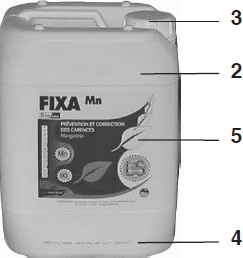
\includegraphics[width=.55\linewidth]{fig_00}
}%figues de la page de garde


\def\xxpied{%
%Cycle 01 -- Modéliser le comportement des systèmes multiphysiques\\
\xxactivite%
}

\setcounter{secnumdepth}{5}
%---------------------------------------------------------------------------

\usepackage{pgfplots}
\begin{document}
%\defimages{images}
%\chapterimage{png/Fond_Cin}
\pagestyle{empty}


%%%%%%%% PAGE DE GARDE COURS
\ifcours
\begin{tikzpicture}[remember picture,overlay]
\node at (current page.north west)
{\begin{tikzpicture}[remember picture,overlay]
\node[anchor=north west,inner sep=0pt] at (0,0) {\includegraphics[width=\paperwidth]{\thechapterimage}};
\draw[anchor=west] (-2cm,-8cm) node [line width=2pt,rounded corners=15pt,draw=ocre,fill=white,fill opacity=0.6,inner sep=40pt]{\strut\makebox[22cm]{}};
\draw[anchor=west] (1cm,-8cm) node {\huge\sffamily\bfseries\color{black} %
\begin{minipage}{1cm}
\rotatebox{90}{\LARGE\sffamily\textsc{\color{ocre}\textbf{\xxnumpartie}}}
\end{minipage} \hfill
\begin{minipage}[c]{14cm}
\begin{titrepartie}
\begin{flushright}
\renewcommand{\baselinestretch}{1.1} 
\Large\sffamily\textsc{\textbf{\xxpartie}}
\renewcommand{\baselinestretch}{1} 
\end{flushright}
\end{titrepartie}
\end{minipage} \hfill
\begin{minipage}[c]{3.5cm}
{\large\sffamily\textsc{\textbf{\color{ocre} \discipline}}}
\end{minipage} 
 };
\end{tikzpicture}};
\end{tikzpicture}


\begin{tikzpicture}[overlay]
\node[shape=rectangle, 
      rounded corners = .25 cm,
	  draw= ocre,
	  line width=2pt, 
	  fill = ocre!10,
	  minimum width  = 2.5cm,
	  minimum height = 3cm,] at (18cm,0) {};
\node at (17.7cm,0) {\rotatebox{90}{\textbf{\Large\color{ocre}{\classe}}}};
%{};
\end{tikzpicture}

\vspace{3.5cm}

\begin{tikzpicture}[remember picture,overlay]
\draw[anchor=west] (-2cm,-6cm) node {\huge\sffamily\bfseries\color{black} %
\begin{minipage}{2cm}
\begin{center}
\LARGE\sffamily\textsc{\color{ocre}\textbf{\xxactivite}}
\end{center}
\end{minipage} \hfill
\begin{minipage}[c]{15cm}
\begin{titrechapitre}
\renewcommand{\baselinestretch}{1.1} 
\Large\sffamily\textsc{\textbf{\xxnumchapitre}}

\Large\sffamily\textsc{\textbf{\xxchapitre}}
\vspace{.5cm}

\renewcommand{\baselinestretch}{1} 
\normalsize\normalfont
\xxcompetences
\end{titrechapitre}
\end{minipage}  };
\end{tikzpicture}
\vfill

\begin{flushright}
\begin{minipage}[c]{.3\linewidth}
\begin{center}
\xxfigures
\end{center}
\end{minipage}\hfill
\begin{minipage}[c]{.6\linewidth}
\startcontents
\printcontents{}{1}{}
\end{minipage}
\end{flushright}

\begin{tikzpicture}[remember picture,overlay]
\draw[anchor=west] (4.5cm,-.7cm) node {
\begin{minipage}[c]{.2\linewidth}
\begin{flushright}

\includegraphics[width=2cm]{png/logoCC}
\end{flushright}
\end{minipage}
\begin{minipage}[c]{.2\linewidth}
\textsl{\xxauteur} \\
\textsl{\classe}
\end{minipage}
 };
\end{tikzpicture}
\newpage
\pagestyle{fancy}

\newpage
\pagestyle{fancy}

\else
\fi


%%%%%%%% PAGE DE GARDE TD
\iftd
%\begin{tikzpicture}[remember picture,overlay]
%\node at (current page.north west)
%{\begin{tikzpicture}[remember picture,overlay]
%\draw[anchor=west] (-2cm,-3.25cm) node [line width=2pt,rounded corners=15pt,draw=ocre,fill=white,fill opacity=0.6,inner sep=40pt]{\strut\makebox[22cm]{}};
%\draw[anchor=west] (1cm,-3.25cm) node {\huge\sffamily\bfseries\color{black} %
%\begin{minipage}{1cm}
%\rotatebox{90}{\LARGE\sffamily\textsc{\color{ocre}\textbf{\xxnumpartie}}}
%\end{minipage} \hfill
%\begin{minipage}[c]{13.5cm}
%\begin{titrepartie}
%\begin{flushright}
%\renewcommand{\baselinestretch}{1.1} 
%\Large\sffamily\textsc{\textbf{\xxpartie}}
%\renewcommand{\baselinestretch}{1} 
%\end{flushright}
%\end{titrepartie}
%\end{minipage} \hfill
%\begin{minipage}[c]{3.5cm}
%{\large\sffamily\textsc{\textbf{\color{ocre} \discipline}}}
%\end{minipage} 
% };
%\end{tikzpicture}};
%\end{tikzpicture}

%%%%%%%%%% PAGE DE GARDE TD %%%%%%%%%%%%%%%
%\begin{tikzpicture}[overlay]
%\node[shape=rectangle, 
%      rounded corners = .25 cm,
%	  draw= ocre,
%	  line width=2pt, 
%	  fill = ocre!10,
%	  minimum width  = 2.5cm,
%	  minimum height = 2.5cm,] at (18.5cm,0) {};
%\node at (17.7cm,0) {\rotatebox{90}{\textbf{\Large\color{ocre}{\classe}}}};
%%{};
%\end{tikzpicture}

% PARTIE ET CHAPITRE
%\begin{tikzpicture}[remember picture,overlay]
%\draw[anchor=west] (-1cm,-2.1cm) node {\large\sffamily\bfseries\color{black} %
%\begin{minipage}[c]{15cm}
%\begin{flushleft}
%\xxnumchapitre \\
%\xxchapitre
%\end{flushleft}
%\end{minipage}  };
%\end{tikzpicture}

% Bandeau titre exo
\begin{tikzpicture}[remember picture,overlay]
\draw[anchor=west] (-2cm,-6cm) node {\huge\sffamily\bfseries\color{black} %
\begin{minipage}{5cm}
\begin{center}
\LARGE\sffamily\color{ocre}\textbf{\textsc{\xxactivite}}

\begin{center}
\xxfigures
\end{center}

\end{center}
\end{minipage} \hfill
\begin{minipage}[c]{12cm}
\begin{titrechapitre}
\renewcommand{\baselinestretch}{1.1} 
\large\sffamily\textbf{\textsc{\xxtitreexo}}

\small\sffamily{\textbf{\textit{\color{black!70}\xxsourceexo}}}
\vspace{.5cm}

\renewcommand{\baselinestretch}{1} 
\normalsize\normalfont
\xxcompetences
\end{titrechapitre}
\end{minipage}  };
\end{tikzpicture}

\else
\fi


%%%%%%%% PAGE DE GARDE FICHE
\iffiche
\begin{tikzpicture}[remember picture,overlay]
\node at (current page.north west)
{\begin{tikzpicture}[remember picture,overlay]
\draw[anchor=west] (-2cm,-3.25cm) node [line width=2pt,rounded corners=15pt,draw=ocre,fill=white,fill opacity=0.6,inner sep=40pt]{\strut\makebox[22cm]{}};
\draw[anchor=west] (1cm,-3.25cm) node {\huge\sffamily\bfseries\color{black} %
\begin{minipage}{1cm}
\rotatebox{90}{\LARGE\sffamily\textsc{\color{ocre}\textbf{\xxnumpartie}}}
\end{minipage} \hfill
\begin{minipage}[c]{14cm}
\begin{titrepartie}
\begin{flushright}
\renewcommand{\baselinestretch}{1.1} 
\large\sffamily\textsc{\textbf{\xxpartie} \\} 

\vspace{.2cm}

\normalsize\sffamily\textsc{\textbf{\xxnumchapitre -- \xxchapitre}}
\renewcommand{\baselinestretch}{1} 
\end{flushright}
\end{titrepartie}
\end{minipage} \hfill
\begin{minipage}[c]{3.5cm}
{\large\sffamily\textsc{\textbf{\color{ocre} \discipline}}}
\end{minipage} 
 };
\end{tikzpicture}};
\end{tikzpicture}


\begin{tikzpicture}[overlay]
\node[shape=rectangle, 
      rounded corners = .25 cm,
	  draw= ocre,
	  line width=2pt, 
	  fill = ocre!10,
	  minimum width  = 2.5cm,
%	  minimum height = 2.5cm,] at (18.5cm,0.5cm) {};
	  minimum height = 2.5cm,] at (18.5cm,0.5cm) {};
\node at (17.7cm,0.5cm) {\rotatebox{90}{\textsf{\textbf{\large\color{ocre}{\classe}}}}};
%{};
\end{tikzpicture}



\else
\fi



\vspace{4.5cm}
\pagestyle{fancy}
\thispagestyle{plain}

\def\columnseprulecolor{\color{white}}
\setlength{\columnseprule}{0.4pt} 

%\defimages2{images}

%\begin{multicols}{2}

\section{Présentation}

Le laboratoire EMSI (Etudes de Mécanique SIsmique) du CEA (Commissariat à l’Energie Atomique) dispose
depuis 1990 de la plus grande table vibrante d’Europe : la table AZALEE (\autoref{fig_01}). Avec ses dimensions de
\SI{6}{m}$\times$\SI{6}{m}, cette table est utilisée pour tester des spécimens de grandes dimensions et de masse importante
(jusqu’à 100 tonnes). Huit vérins hydrauliques, pouvant développer chacun une force maximale dynamique de
100 tonnes, permettent de réaliser des excitations tridimensionnelles.

\begin{multicols}{2}
\begin{figure}[H]
\centering
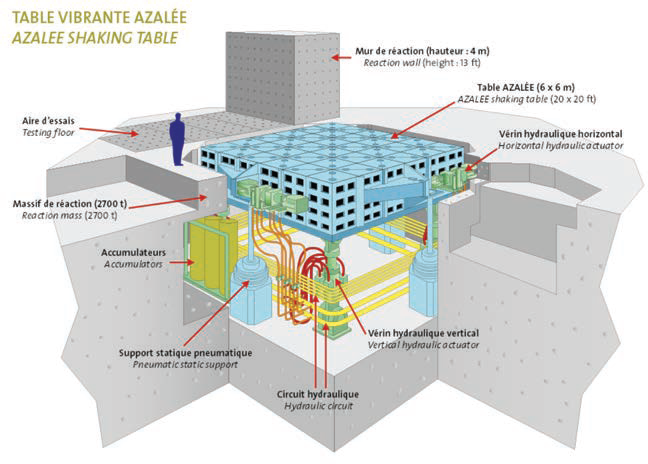
\includegraphics[width=\linewidth]{fig_01}
\caption{Table vibrante AZALEE \label{fig_01}}
\end{figure}

\begin{figure}[H]
\centering
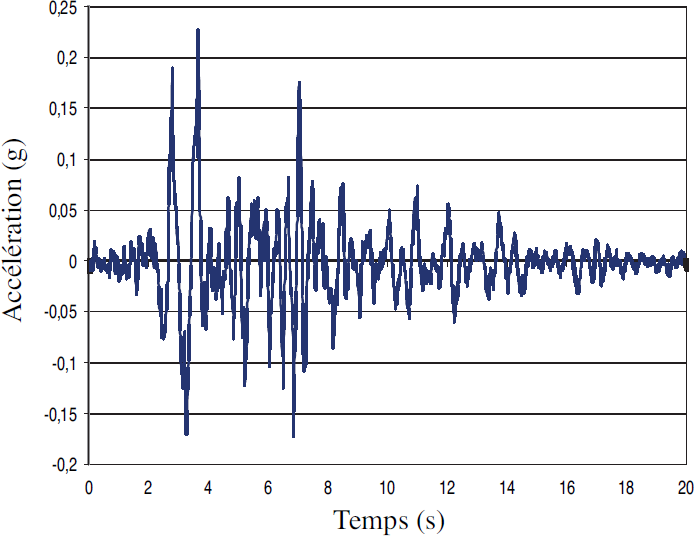
\includegraphics[width=\linewidth]{fig_02}
\caption{Enregistrement d’un séisme à Kobe, au Japon (accélération dans une des trois directions, exprimée en~g) \label{fig_02}}
\end{figure}

\end{multicols}

L’étude des effets d’un séisme sur une structure est encore trop complexe pour pouvoir être abordée sans
un appui expérimental dédié, qui vient en renfort des simulations numériques. La table AZALEE permet de
reproduire expérimentalement le mouvement du sol ou du plancher d’un bâtiment sur lequel repose la structure.
Ce mouvement est issu d’enregistrements de séismes réels qui ont eu lieu dans les zones sismiques un peu
partout dans le monde (exemple d’un séisme à Kobe, au Japon, \autoref{fig_02}). La \autoref{fig_03} représente la table avec une maquette de bâtiment en béton armé, qui va subir une reproduction de séisme à l’aide des vérins. L’ensemble
est, entre autres, muni de 92 accéléromètres, 50 capteurs de déplacement et 43 jauges de déformations, qui
serviront pour l’analyse de la réponse. Une étude de ce type nécessite environ 3 années de travail (depuis
la préparation de la campagne d’essais jusqu’à l’évacuation de la maquette), auxquelles s’additionne tout le
dépouillement des données !


\begin{figure}[H]
\centering
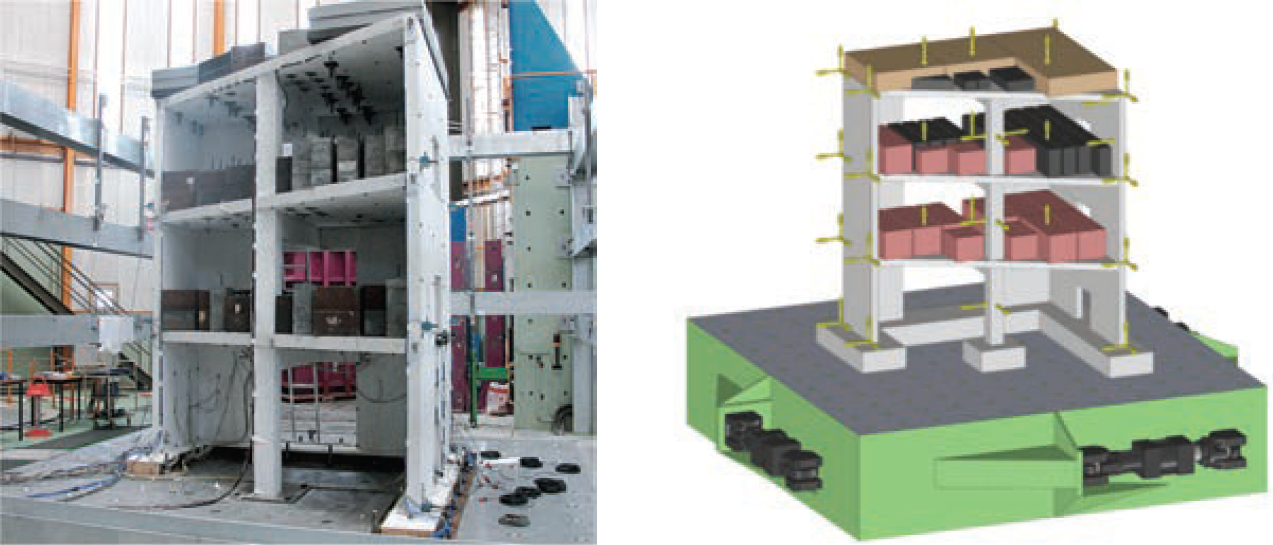
\includegraphics[width=\linewidth]{fig_03}
\caption{Table AZALEE avec une << maquette >> de \SI{9}{m} de haut d’un bâtiment en béton armé \label{fig_03}}
\end{figure}


\section{Etude de l’exigence << Fournir à la table les mouvements caractéristiques d’un séisme~>>}

\begin{obj}
On s’intéresse à l’exigence << Fournir à la table des mouvements caractéristiques d’un séisme~>>.
Plus précisément, on va s’intéresser à la cinématique de la table AZALEE assurant des mouvements représentatifs de ceux d’un sol (exigence << Permettre un mouvement libre >>), ainsi qu’aux actions mécaniques que doivent pouvoir développer les vérins pour assurer des accélérations compatibles avec des essais sismiques (exigence << Fournir la puissance nécessaire >>). Le tableau suivant précise les critères et niveaux associés à ces exigences (le $g$ est ici l’unité d’accélération : $\SI{1}{g} = \SI{9, 81}{m.s^{-2}}$).
\end{obj}

\subsection{Modélisation simplifiée d’une structure soumise à un séisme}

Pour comprendre les phénomènes mis en jeu lors d’un séisme, on se propose d’utiliser le modèle très simplifié
de la \autoref{fig_05}. La structure (le bâtiment de la \autoref{fig_03}) est modélisée par 4 poutres, encastrées au niveau du sol (fondations) et supportant un toit. Les poutres sont supposées pouvoir fléchir sous l’effet des vibrations du sol, tandis que le toit est infiniment rigide.



\begin{figure}[H]
\centering
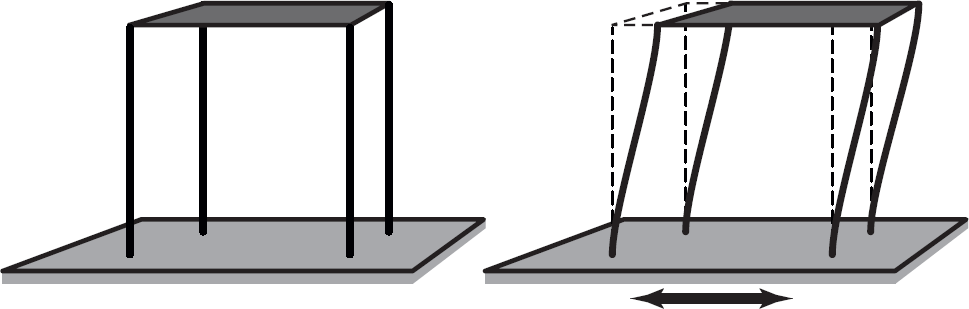
\includegraphics[width=0.7\linewidth]{fig_05}
\caption{Modèle de la structure testée, au repos et en mouvement sous l’influence des
déplacements du sol \label{fig_05}}
\end{figure}


On s’intéresse maintenant à la structure de la \autoref{fig_06} (droite), constituée de 4 poutres identiques à la
précédente (seules les deux poutres au premier plan sont représentées), supportant le toit indéformable de
masse $m$. On néglige les effets d’inertie sur les poutres devant la dynamique du toit, dont la position est repérée à l’aide du paramètre y par rapport au sol, considéré comme un reférentiel galiléen.

On note $\vect{F}=-F\vect{y} = -ky  \vect{y}$ l'action  d'une poutre sur la table, $k$ étant la raideur en flexion d'une poutre.
\begin{figure}[H]
\centering
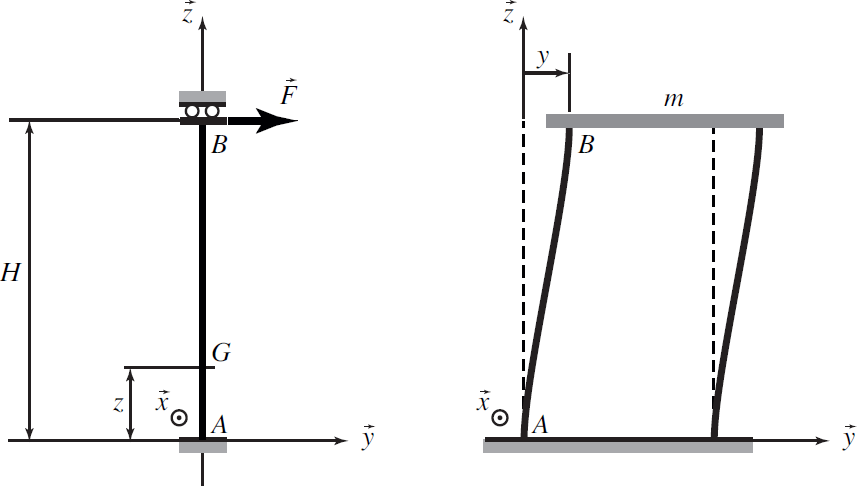
\includegraphics[width=.7\linewidth]{fig_06}
\caption{Etude de la flexion d’une des 4 poutres, puis de l’ensemble \label{fig_06}}
\end{figure}



\subparagraph{\label{q_02}}\textit{Donner l’équation du mouvement qui régit la dynamique de la table dans son mouvement par rapport au sol lorsqu’elle n’est soumise à aucune sollicitation extérieure.}
\ifprof
\begin{corrige} ~\\

\end{corrige}
\else
\fi

On suppose maintenant que le sol est en mouvement, du fait d’un séisme, et le référentiel associé ne peut
donc plus être considéré comme galiléen. La \autoref{fig_07} introduit cette distinction entre le référentiel terrestre
(repère associé $\left(O,\vect{x_0},\vect{y_0},\vect{z_0}\right)$), supposé galiléen, et le référentiel lié au sol (repère associé $\left(A,\vect{x},\vect{y},\vect{z}\right)$). Le sol
est animé d’un mouvement de translation par rapport au référentiel galiléen, mais non uniforme car $\vect{OA}$ est régi
par des signaux du type de celui représenté sur la \autoref{fig_02}.
Pour fixer les idées, on suppose un signal simple, tel que $\vect{OA}=Y_s(t)\vect{y_0}$ avec 
$Y_s (t) = A_s \sin\left(\omega_s t\right)$ où $A_s$ est
l’amplitude et $\omega_s$ la pulsation du signal sismique.

\subparagraph{\label{q_03}}\textit{Donner l’équation du mouvement qui régit la dynamique de la table dans son mouvement par rapport au sol lorsqu’elle n’est soumise à aucune sollicitation extérieure. On exprimera cette relation sous l a forme $\dfrac{\dd^2 y(t)}{\dd t}+\omega^2 y(t) = f(t)$ et on précisera les expressions de $\omega$ et $f(t)$ en fonction des données du problème.}
\ifprof
\begin{corrige} ~\\

\end{corrige}
\else
\fi


\begin{figure}[H]
\centering
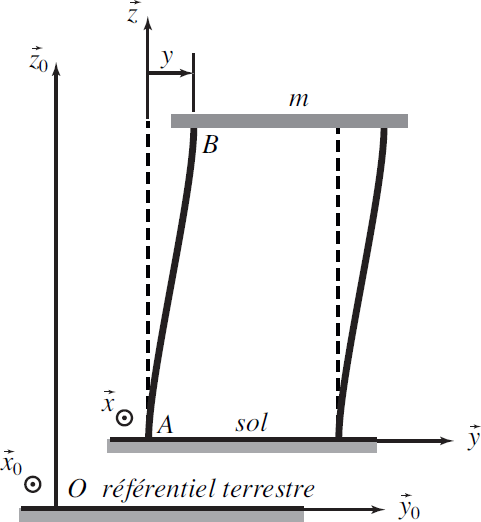
\includegraphics[width=.5\linewidth]{fig_07}
\caption{Mouvement du sol dû à un séisme\label{fig_07}}
\end{figure}


\section{Modélisation du comportement temporel des éléments de la chaîıne de transmission de puissance}

\begin{obj}
L’objectif de cette partie est de définir un modèle permettant d’appréhender suffisamment
précisément le comportement dynamique de la chaîne de transmission de puissance afin de définir dans la partie
suivante les correcteurs permettant de valider les crirères de comportement imposés par le cahier des charges.
Afin de simplifier les calculs, un modèle de vérin équivalent aux quatre vérins verticaux sera mis en place.
\end{obj}


\begin{figure}[H]
\centering
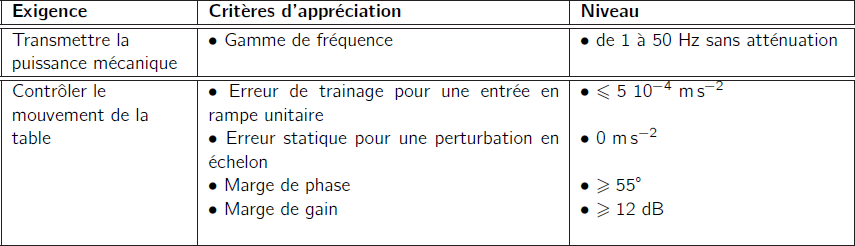
\includegraphics[width=0.7\linewidth]{req_01}
%\caption{TABLEAU EXIGENCES \label{req_01}}
\end{figure}

\subsection{Analyse préliminaire}

\subsubsection{Description du cadre de l’étude et hypothèses}

On s’intéresse uniquement dans cette partie au déplacement vertical de la table sismique. L’architecture
simplifiée du système dans ce cadre particulier est précisée sur le schéma (\autoref{fig_13}). Le calculateur détermine
le signal de consigne en accélération verticale $a_c (t)$ en fonction de la sollicitation que l’on souhaite donner à
la structure. Ce signal est converti en une tension de consigne $u_c (t)$. À partir de cette tension de consigne et
de la mesure des accéléromètres placés sur la table sismique, un régulateur électronique génère une tension
d’alimentation des servo-valves qui délivrent alors un débit $q(t)$ aux quatre vérins verticaux. Le mouvement des
tiges des vérins est alors transmis à la table sismique via les rotules.

La table sismique est supposée infiniment rigide dans toute la suite du sujet. $P_e(t)$ correspond aux efforts
pouvant perturber le mouvement vertical de la table lors de l’essai.


\begin{figure}[H]
\centering
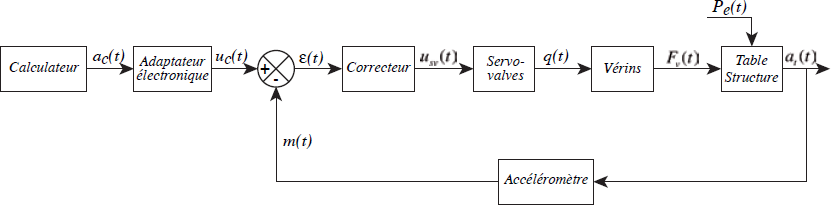
\includegraphics[width=\linewidth]{fig_13}
\caption{Architecture simplifiée du système -- cas d’un mouvement vertical \label{fig_13}}
\end{figure}


\subsubsection{Détermination du comportement attendu du système}

Les signaux de consigne correspondant à un tremblement de terre (\autoref{fig_02}) ont un contenu fréquentiel
situé entre 1 et \SI{50}{Hz}. Il est donc indispensable que le système soit en mesure de transmettre à un point de
la table sismique un mouvement correspondant à ce type de consigne et ce, sur toute la gamme de fréquence
nécessaire.

\subparagraph{\label{q_}}\textit{Proposer un modèle pour le comportement souhaité de l’ensemble du système (comprenant l’ensemble de la partie hydraulique, des pièces mécaniques et des contrôleurs électroniques).
Préciser si c’est un filtre <<~passe ~>>,  <<~passe ~>> ou <<~passe bande~>> et donner les
caractéristiques de ce filtre.}
\ifprof
\begin{corrige} ~\\

\end{corrige}
\else
\fi


On considère le schéma-blocs de la \autoref{fig_13}.

\subparagraph{\label{q_}}\textit{À partir des caractéristiques du filtre proposé, donner, en la justifiant, la valeur de la pulsation à \SI{0}{dB} de la FTBO (telle que $M(p) = \text{FTBO}(p)\varepsilon(p)$) de l’asservissement proposé.}
\ifprof
\begin{corrige} ~\\

\end{corrige}
\else
\fi


Quelle que soit la valeur proposée, on prendra pour la suite $\omega_{\SI{0}{dB}} = \SI{1000}{rad.s^{-1}}$.

\subsection{Modélisation du comportement dynamique des composants}

\subsubsection{Détermination des fonctions de transfert des servo-valves}

Les servo-valves utilisées sont relativement complexes. Elles sont composées de 3 étages et l’étude de leur
comportement dépasse largement le cadre de ce sujet. Aussi, dans un premier temps, nous allons considérer
que leur dynamique est suffisante pour modéliser leur comportement par des gains purs $K_{\text{sv}}$ avec :
$K_{\text{sv}} = \SI{2e-4}{m^3s^{-1}V^{-1}}$.


\subparagraph{\label{q_}}\textit{En considérant les débits maximum des vérins verticaux et des servo-valves précisés en Annexe
B, déterminer le nombre de servo-valves nécessaires pour alimenter chaque vérin puis préciser
l’expression de la fonction de transfert $H_{\text{sv 1}}(p)$ en fonction de $K_{\text{sv}}$ (\autoref{fig_14}).}
\ifprof
\begin{corrige} ~\\

\end{corrige}
\else
\fi


\begin{figure}[H]
\centering
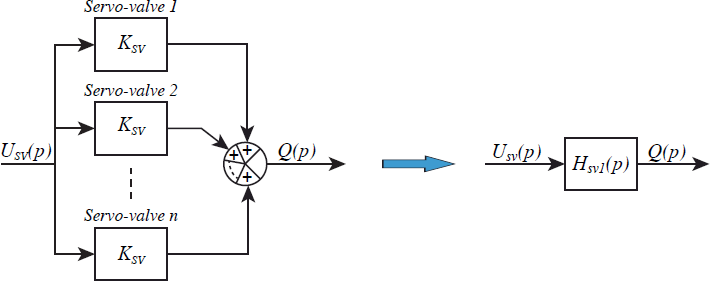
\includegraphics[width=0.7\linewidth]{fig_14}
\caption{n servo-valves alimentant 1 vérin \label{fig_14}}
\end{figure}


\subsubsection{Détermination d’un modèle équivalent au comportement des 4 vérins}

Dans cette partie, nous allons nous attacher à déterminer le modèle d’un unique vérin équivalent au comportement
des quatre vérins verticaux.

\paragraph{Modélisation du comportement avec un seul vérin}

On considère dans un premier temps que la table n’est déplacée qu’avec un seul vérin vertical (\autoref{fig_15}).

\begin{figure}[H]
\centering
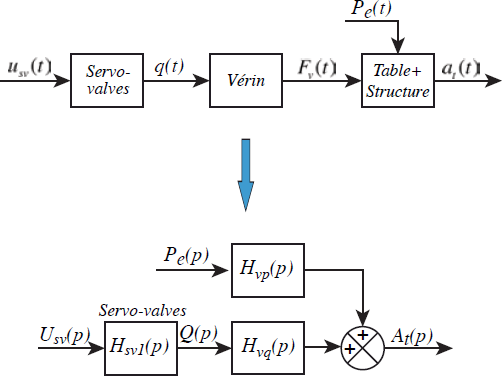
\includegraphics[width=0.6\linewidth]{fig_15}
\caption{Table déplacée par 1 seul vérin - Schémas-blocs dans le domaine temporel et dans
le domaine symbolique \label{fig_15}}
\end{figure}

\paragraph{Equations caractéristiques avec un modèle de fluide compressible}

La compressibilité du fluide étant prise en compte dans le modèle, l’évolution du débit est une fonction du
déplacement de la tige du vérin mais aussi de la pression du fluide sous la forme de la relation (1). L’effort
exercé par le vérin en sortie de tige est décrit par la relation (2) :
$$q(t)=S\dfrac{\dd \lambda(t)}{\dd t}+\dfrac{V_0}{2B}\dfrac{\dd p_r(t)}{\dd t} \quad (1) 
\quad \quad  \text{et} \quad \quad
F_v(t)=Sp_r(t) \quad (2) $$

où :
\begin{itemize}
\item $p_r(t)$ : pression utile dans le vérin;
\item $V_0$ : volume caractéristique moyen de fluide contenu dans le vérin et les durites, $V_0 = \SI{5e-3}{m^3}$ ;
\item $B$ : coefficient de compressibilité du fluide, $B = \SI{0,5e9}{Pa}$ ;
\item $F_v (t)$ : effort développé par le vérin en sortie de tige ;
\item $S$ : section utile du vérin, $S = \SI{500}{cm^2}$ ;
\item $\lambda(t)$ : déplacement vertical de la table.
\end{itemize}
On a de plus $a_t(t) = \dfrac{\dd^2 \lambda(t)}{\dd t^2}$.




\subparagraph{\label{q_20}}\textit{Appliquer la transformation de Laplace aux équations précédentes. Recopier et remplir les cases grisées du schéma-blocs ci-dessous.}
%et compléter les parties grisées du schéma-blocs du Cahier Réponses.}
\ifprof
\begin{corrige} ~\\

\end{corrige}
\else
\begin{figure}[H]
\centering
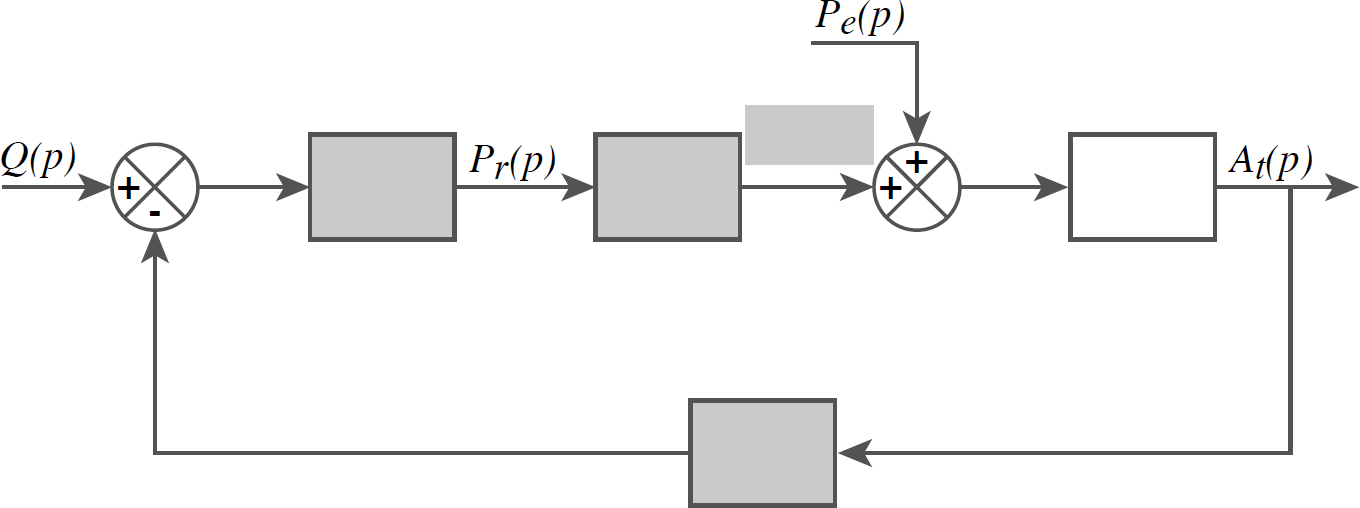
\includegraphics[width=0.6\linewidth]{q_20}
\end{figure}
\fi



\paragraph{Modélisation du comportement dynamique de la table}

On considère uniquement le cas d’un mouvement de translation verticale dans le cas d’une charge maximale
fixée sur la table sismique.

\subparagraph{\label{q_}}\textit{Déterminer l’expression de l’équation de mouvement de la table et la mettre sous la forme $Ma_t(t) = F_v (t) + P_e(t)$. Compléter la case blanche du schéma-blocs ci-dessus 
%Compléter la partie grisée du schéma-blocs du Cahier Réponses
caractérisant le comportement d’un vérin hydraulique en mentionnant les expressions de la
masse $M$ et de la perturbation $P_e(p)$ en fonction des masses de la table $M_t$ et du spécimen
$M_s$.}
\ifprof
\begin{corrige} ~\\

\end{corrige}
\else
\fi

\paragraph{Détermination des fonctions de transfert d’un vérin}

\subparagraph{\label{q_}}\textit{Déterminer les expressions des fonctions de transfert en boucle fermée du vérin $H_{\text{vq}}$ et $H_{\text{vp}}$ (telles que $A_t(p)=H_{\text{vq}}(p) Q(p)+H_{\text{vp}}(p) P_e(p)$) et préciser les expressions des coefficients $K_v$ , $K_p$ et $\omega_v$ de leurs formes canoniques : $H_{\text{vq}}(p)=\dfrac{K_v p}{1+\dfrac{p^2}{\omega_v^2}}$ et $H_{\text{vp}}(p)=\dfrac{K_p p^2}{1+\dfrac{p^2}{\omega_v^2}}$.}
\ifprof
\begin{corrige} ~\\

\end{corrige}
\else
\fi

\paragraph{Modélisation du comportement équivalent à deux vérins}

On considère ici que la table est soumise à l’action de deux vérins (\autoref{fig_16}). Pour chaque vérin $i$ , nous
avons les équations suivantes :
$q_i(t)=S\dfrac{\dd \lambda(t)}{\dd t}+\dfrac{V_0}{2B}\dfrac{\dd p_{r_i}(t)}{\dd t} \quad (1) 
\quad \quad  \text{et} \quad \quad
F_{v_i}(t)=Sp_{r_i}(t) \quad (2) $
où :
\begin{itemize}
\item $p_{r_i} (t)$ : pression utile dans le vérin $i$;
\item $F_{v_i} (t)$ : effort développé par le vérin $i$ en sortie de tige.
\end{itemize}

\begin{figure}[H]
\centering
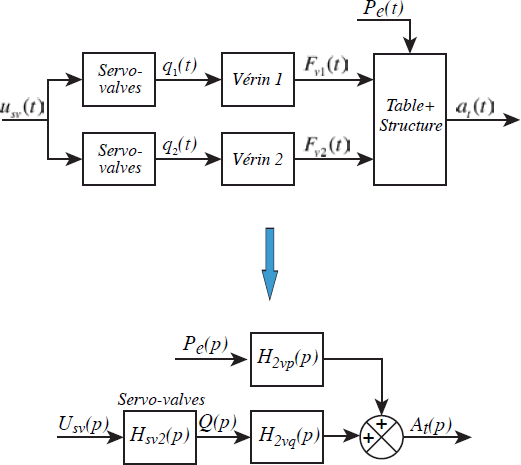
\includegraphics[width=0.6\linewidth]{fig_16}
\caption{Table déplacée par 2 vérins - Schémas-blocs dans le domaine temporel et dans le
domaine symbolique \label{fig_16}}
\end{figure}

\subparagraph{\label{q_23}}\textit{En utilisant les équations précédentes, compléter les parties grisées du schéma-blocs du Document Réponses.}
\ifprof
\begin{corrige} ~\\

\end{corrige}
\else
\fi

\paragraph{Modélisation du comportement dynamique de la table}
On considère uniquement le cas d’un mouvement de translation verticale dans le cas d’une charge maximale
fixée sur la table sismique. On considère de plus que les mouvements des 2 vérins verticaux sont parfaitement
synchronisés.


\subparagraph{\label{q_24}}\textit{Déterminer l’expression de l’équation de mouvement de la table. Compléter la partie blanche à la droite du schéma-blocs du Document Réponses caractérisant le comportement de deux vérins hydrauliques
en mentionnant les expressions de la masse $M$ et de la perturbation $P_e(p)$ en fonction des
masses de la table $M_t$ et du spécimen $M_s$.}
\ifprof
\begin{corrige} ~\\

\end{corrige}
\else
\fi

\paragraph{Détermination des fonctions de transfert avec 2 vérins}

\subparagraph{\label{q_25}}\textit{Déterminer les expressions des fonctions de transfert en boucle fermée du vérin $H_{\text{vq1}}$, $H_{\text{vq2}}$ et $H_{\text{vp}}$ telles que $A_t(p)=H_{\text{vq1}}(p) Q_1(p)+H_{\text{vq2}}(p) Q_2(p)+H_{\text{vp}}(p) P_e(p)$.}
\ifprof
\begin{corrige} ~\\

\end{corrige}
\else
\fi


\subparagraph{\label{q_26}}\textit{En supposant que les débits $q_1(t)$ et $q_2(t)$ sont identiques ($q_1(t)=q_2(t)=q(t)$) déterminer les expressions des fonctions de transfert $H_{2vq}$ telle que $A_t(p)=H_{2\text{vq}}(p) Q(p)+H_{\text{2\text{vp}}}(p) P_e(p)$. Préciser les expressions des coefficients $K_{2v}$ , $K_{2p}$ et $\omega_{2v}$ de leurs formes canoniques : $H_{\text{2\text{vq}}}(p)=\dfrac{K_{2v} p}{1+\dfrac{p^2}{\omega_{2v}^2}}$ et $H_{\text{2\text{vp}}}(p)=\dfrac{K_{2p} p^2}{1+\dfrac{p^2}{\omega_{2v}^2}}$. 
Donner les expressions de $S_{\text{eq}_{2v}}$ et de $M_{eq_{2v}}$ de telle sorte que les expressions de $K_{2v}$ et 
$\omega_{2v}$ en fonction $S_{\text{eq}_{2v}}$ et $M_{eq_{2v}}$ 
correspondent à celles de $K_v$ et $\omega_v$ en fonction de $S$ et $M$.} 
\ifprof
\begin{corrige} ~\\

\end{corrige}
\else
\fi



\subparagraph{\label{q_27}}\textit{Déterminer l’expression de la fonction de transfert $H_{\text{sv}2}(p)$ en fonction de $K_{\text{sv}}$, $H_{\text{sv}2}(p)$ représentant la fonction de transfert modélisant le comportement des servo-valves nécessaires à l’alimentation en fluide des 2 vérins.}
\ifprof
\begin{corrige} ~\\

\end{corrige}
\else
\fi

\paragraph{Détermination des fonctions de transfert avec 4 vérins}

\subparagraph{\label{q_28}}\textit{Par extension, donner les expressions de $S_{\text{eq4v}}$ , de $M_{\text{eq4v}}$ et de $H_{\text{sv4}}(p)$.}
\ifprof
\begin{corrige} ~\\

\end{corrige}
\else
\fi

\subsubsection{Fonction de transfert de l’adaptateur électronique d’entrée}

L’accéléromètre est supposé avoir un temps de réponse suffisamment petit afin de modéliser son comportement
par un gain pur : $H_{\text{ac}} (p) = C$ avec $C = \SI{0,2}{Vm^{-1} s^2}$.

Le temps de réponse de l’adaptateur électronique est suffisamment faible comparativement aux temps
caractéristiques des autres systèmes pour que l’on puisse modéliser son comportement temporel par un gain
pur $H_{\text{ae}} (p)=K_{\text{ae}}$.


\subparagraph{\label{q_29}}\textit{À l’aide de la \autoref{fig_17}, donner l’expression de $K_{\text{ae}}$ pour qu’une erreur nulle en régime
permanent conduise à un écart nul en régime permanent.}
\ifprof
\begin{corrige} ~\\

\end{corrige}
\else
\fi



\begin{figure}[H]
\centering
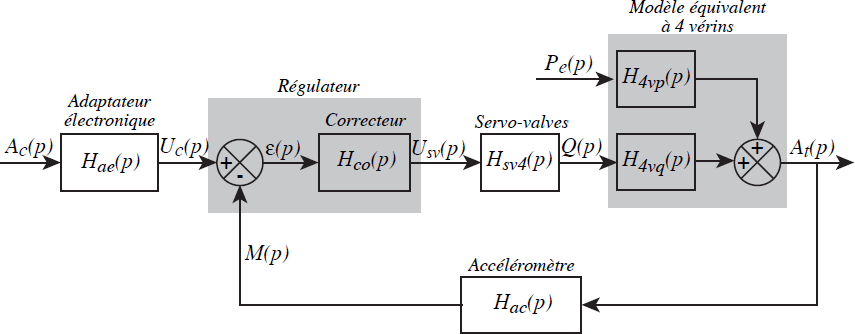
\includegraphics[width=0.7\linewidth]{fig_17}
\caption{Architecture générale du contrôle du mouvement de la table \label{fig_17}}
\end{figure}


Quels que soient les résultats obtenus précédemment, on considèrera dans la suite de cette partie :
$$
H_{\text{4vq}}(p)=\dfrac{K_{\text{4v}}p}{1+\dfrac{p^2}{\omega^2_{\text{4v}}}} 
\quad \quad
H_{\text{4vp}}(p)=\dfrac{K_{\text{4p}}p^2}{1+\dfrac{p^2}{\omega^2_{\text{4v}}}} 
\quad \quad
H_{\text{sv4}}(p)=K_s.
$$

Avec 
$K_{\text{4v}}=\SI{2}{m^{-2}}$,
$\omega_{\text{4v}}=\SI{1500}{rad.s^{-1}}$
et $K_s = \SI{25e-4}{m^3s^{-1}V^{-1}}$.


Afin de vérifier dans un premier temps les critères de précision du cahier des charges, on place un premier
correcteur de type intégral : $H_{\text{CO}}(p)=\dfrac{K_{\text{CO}}}{p^\alpha}$.


\subparagraph{\label{q_30}}\textit{Préciser, en la justifiant, la valeur minimale de $\alpha$ qui permet de vérifier les critères d’erreur en poursuite et d’erreur vis à vis de la perturbation.}
\ifprof
\begin{corrige} ~\\

\end{corrige}
\else
\fi

\subparagraph{\label{q_31}}\textit{En prenant $K_{\text{CO}}=1$, donner l’expression de la Fonction de Transfert en Boucle Ouverte de
l’asservissement proposé, puis représenter son diagramme de Bode asymptotique sur le document réponse.}
\ifprof
\begin{corrige} ~\\

\end{corrige}
\else
\fi

\subparagraph{\label{q_32}}\textit{Déterminer la valeur minimale de $K_{\text{CO}}$ qui permet de vérifier le critère sur la pulsation à \SI{0}{dB} de la FTBO.}
\ifprof
\begin{corrige} ~\\

\end{corrige}
\else
\fi

\subparagraph{\label{q_33}}\textit{Sur le diagramme de Bode du Document Réponse de la question \ref{q_31}, représenter l’allure du
diagramme de Bode réel de la FTBO. Préciser, en le justifiant, si le comportement est stable.}
\ifprof
\begin{corrige} ~\\

\end{corrige}
\else
\fi

\subsubsection{Comportement dynamique avec prise en compte d’un débit de fuite}

On considère ici le modèle équivalent aux quatre vérins obtenus précédemment. Pour pallier le problème de
stabilité du modèle précédemment établi, une solution possible consiste à introduire un débit de fuite au niveau
des vérins. Celui-ci a pour effet de réduire artificiellement le débit réel entrant dans les vérins en fonction de la
pression utile. L’expression du débit est alors :
$q(t)=S_{\text{eq4v}}\dfrac{\dd \lambda(t)}{\dd t}+\dfrac{V_0}{2B}\dfrac{\dd p_{r}(t)}{\dd t} +\delta p_{r}(t)$ où $\delta$ représente le coefficient de débit de fuite.


\subparagraph{\label{q_34}}\textit{Proposer une modification du schéma-blocs suivant
%donné sur le Cahier Réponses 
afin de prendre en compte le débit de fuite.
Déterminer l’expression de la fonction de transfert $H_{\text{4v2}}$ (telle que $A_t(p) = H_{\text{4v2}}(p) Q(p)$)
associée au comportement dynamique du vérin équivalent ainsi modélisé. On donnera le
résultat sous la forme suivante : $H_{\text{4v2}}(p)=\dfrac{K_{\text{4v}}p}{1+a_1 p + \dfrac{p^2}{\omega_{4v}^2}}$.
Donner l’expression de $a_1$ en fonction de $M_{\text{eq4v}}$, $\delta$ et $S_{\text{eq4v}}$, et déterminer l’expression du coefficient d’amortissement $\xi_v$ ($a_1 =\dfrac{2\xi_v}{\omega_{4v}}$) du second ordre du dénominateur de $H_{\text{4v2}}(p)$ en
fonction de $M_{\text{eq4v}}$ , $\delta$, $S_{\text{eq4v}}$ , $B$ et $V_0$.
}
\ifprof
\begin{corrige} ~\\

\end{corrige}
\else

\begin{figure}[H]
\centering
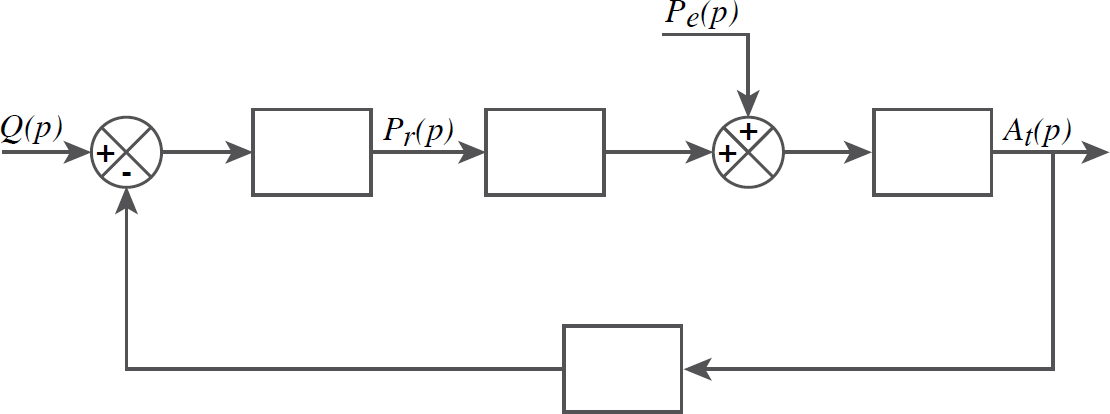
\includegraphics[width=0.7\linewidth]{q_34}
%\caption{Architecture générale du contrôle du mouvement de la table \label{fig_17}}
\end{figure}

\fi

\subsubsection{Analyse du comportement global et détermination de la valeur limite du coefficient
de débit de fuite}

L’objectif de cette partie est d’analyser le comportement dynamique prévu par le modèle développé précédemment.
Pour cela, on considère le système modélisé par le schéma-blocs de la \autoref{fig_17}.

\subparagraph{\label{q_35}}\textit{Déterminer la valeur limite de $\xi_v$ assurant le critère de stabilité imposé dans le cahier des
charges. En déduire la valeur numérique limite du coefficient de débit de fuite $\delta$ puis celle du
débit de fuite à pression maximale. Conclure quant à la capacité des servo-valves à permettre
le débit total lors d’un déplacement à vitesse maximale de la tige du vérin.}
\ifprof
\begin{corrige} ~\\

\end{corrige}
\else
\fi

Le problème de fond ici est lié au fait que la pulsation propre $\omega_{4v}$ du mode de second ordre de la fonction
de transfert du vérin est trop proche de la pulsation à \SI{0}{dB} souhaitée de la FTBO pour garantir une dynamique
suffisante du système bouclé. On souhaite donc augmenter la valeur de la pulsation propre $\omega_{4v}$ afin de garantir
au moins une décade d’écart avec la pulsation à \SI{0}{dB} de la Fonction de Transfert en Boucle Ouverte du système.

\subparagraph{\label{q_36}}\textit{Quelle valeur de diamètre du vérin permet de vérifier la condition précédente. Cette valeur
est-elle réaliste ?}
\ifprof
\begin{corrige} ~\\

\end{corrige}
\else
\fi

\section{Validation des critères principaux
de l’exigence << Contrôler les
mouvements de la table >>}
\begin{obj}
L’objectif de cette partie est de définir la correction complète et de déterminer les valeurs
numériques des paramètres caractéristiques des différents correcteurs, afin d’obtenir un asservissement de
l’accélération de la table validant les critères de la fonction technique << Contrôler les mouvements de la table>>.
Le tableau suivant précise les critères et niveaux associés à cette exigence.
\end{obj}


\begin{figure}[H]
\centering
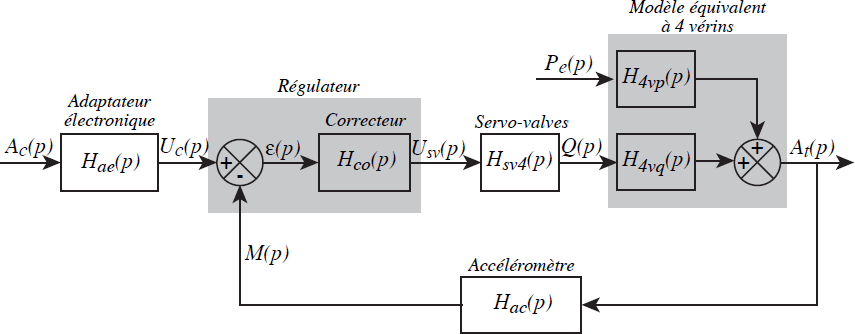
\includegraphics[width=0.7\linewidth]{fig_17}
\caption{Exigences \label{req_02}}
\end{figure}

\subsection{Synthèse des résultats obtenus précédemment}

On considère le schéma-blocss de la \autoref{fig_18} avec :

$$
H_{\text{ac}}(p)=C
\quad \quad
H_{\text{sv4}}(p)=K_s
\quad \quad
H_{\text{4vq}}(p)=\dfrac{K_{\text{4v}}p}{1+2\dfrac{\xi_v}{\omega_{\text{4v}}}p+\dfrac{p^2}{\omega^2_{\text{4v}}}}.
$$


\begin{figure}[H]
\centering
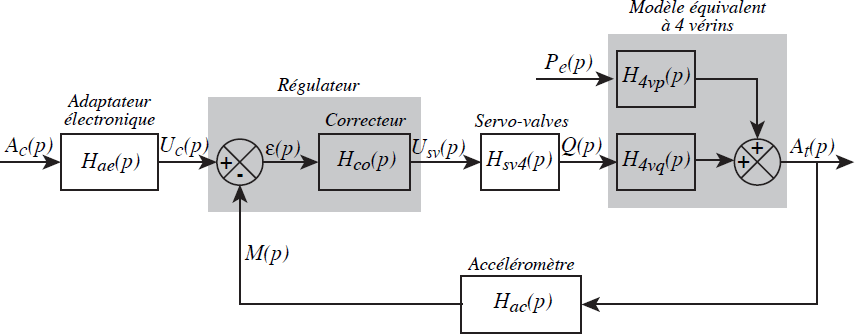
\includegraphics[width=0.7\linewidth]{fig_18}
\caption{Architecture générale du contrôle du mouvement de la table \label{fig_18}}
\end{figure}

Quels que soient les résultats obtenus précédemment, on prendra les valeurs numériques suivantes
$K_{\text{4v}}=\SI{2}{m^{-2}}$,
et $K_s = \SI{25e-4}{m^3s^{-1}V^{-1}}$.

\subsection{Détermination des caractéristiques d’un filtre de second ordre}


Nous avons vu dans la partie précédente qu'il n'était pas perinent de régler le problème de comportement du système en jouant sur les caractéristiques matérielles telles que le diamètre des pistons des vérins ou le débit de fuite des vérins. Nous nous tournons donc vers l’utilisation de filtres électroniques afin d’éloigner la pulsation
propre du système du second ordre de la pulsation à \SI{0}{dB} précisée dans le cahier des charges. On souhaite donc
augmenter la valeur de la pulsation propre du système du second ordre afin de garantir au moins deux décades
d’écart avec la pulsation à \SI{0}{dB} de la Fonction de Transfert en Boucle Ouverte du système. On considère alors
un filtre électronique du second ordre de type Notch de fonction de transfert : $H_N(p)=\dfrac{1+\dfrac{2\xi_n}{\omega_n}p+\dfrac{p^2}{\omega_n^2}}{1+\dfrac{2\xi_d}{\omega_d}p+\dfrac{p^2}{\omega_d^2}}$.

Le réglalge optimum du correcteur doit compenser parfaitement le mode de second ordre de la fonction de
transfert du vérin. Pour cela, on effectue un essai afin d’identifier les caractéristiques de ce mode. Aucun
réglage spécifique du debit de fuite n’a été réalisé, la compensation du mode rendant inutile cette étape.

Une tension de commande $u_{\text{sv}} (t) = e_0u(t)$ (avec $u(t)$ l’échelon unitaire) est envoyée en entrée des servovalves.
La tension délivrée par l’accéleromètre vertical est numérisée. Afin d’identifier les caractéristiques du second
ordre on décide d’intégrer numériquement les mesures données par l’accéléromètre afin de tracer l’évolution
la vitesse verticale de la table en fonction du temps. L’obtention de la vitesse à partir de l’accélération
ecessite donc la réalisation d’une intégration numérique. Les données obtenues lors de l’essai sont stockées
dans 2 listes de flottants de même longueur : $U_{\text{acc}}$ pour la tension image de l'accélération de la table et $T$ pour le temps.

Le résultat obtenu après intégration numérique est donné sur la \autoref{fig_19}.


\begin{figure}[H]
\centering
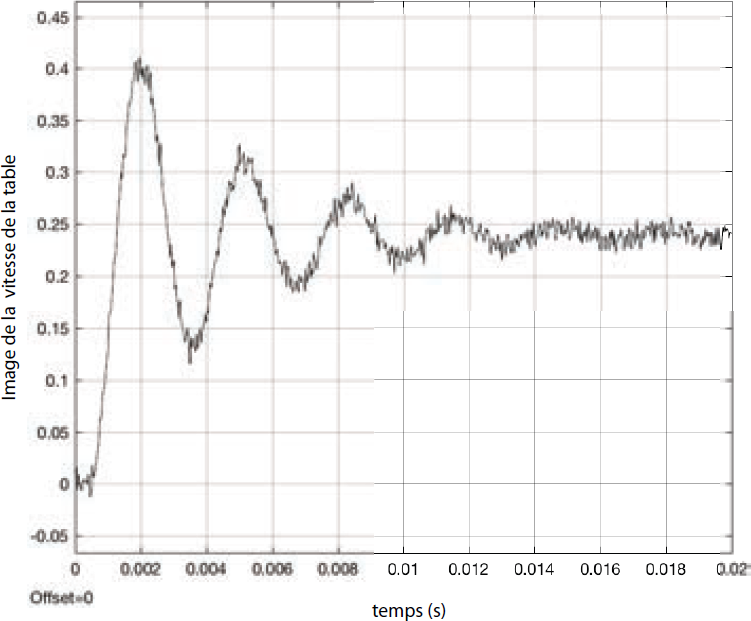
\includegraphics[width=0.55\linewidth]{fig_19}
\caption{Image de la vitesse de la table après intégration numérique \label{fig_19}}
\end{figure}



\subparagraph{\label{q_39}}\textit{À l’aide du graphe de la \autoref{fig_19} et de l’annexe A, déterminer les valeurs numériques
expérimentales de $\omega_{\text{4v}}$ et $\xi_v$ . Vous effectuerez les tracés utiles, avec le plus grand soin, sur
les graphes du Document Réponses.}
\ifprof
\begin{corrige} ~\\

\end{corrige}
\else
\fi

\subparagraph{\label{q_40}}\textit{Quels inconvénients sur le comportement réel du système peuvent découler de cette méthode
consistant à vouloir compenser le mode de second ordre de la fonction de transfert du vérin
par ce type de filtre électronique ? Que cela implique-t-il sur la méthodologie de réalisation
des essais sur différentes structures ?}
\ifprof
\begin{corrige} ~\\

\end{corrige}
\else
\fi

\subsection{Détermination complète de la correction}
On suppose que le numérateur du filtre Notch compense parfaitement le mode de second ordre de la fonction
de transfert du vérin. On adopte les caractéristiques suivantes pour le dénominateur :
\begin{itemize}
\item $\omega_d = \SI{100 000}{rad.s^{-1}}$ ;
\item $\xi_d = 1$.
\end{itemize}
On ne s’intéresse par la suite qu’à l’étude du comportement vis à vis de la consigne. On obtient alors le
schéma de la \autoref{fig_20}, schéma qui donne celui de la \autoref{fig_21} après simplification.

\begin{figure}[H]
\centering
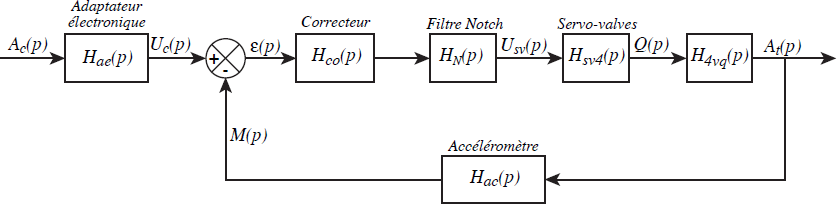
\includegraphics[width=0.8\linewidth]{fig_20}
\caption{ Architecture simplifiée du contrôle du mouvement de la table \label{fig_20}}
\end{figure}


\begin{figure}[H]
\centering
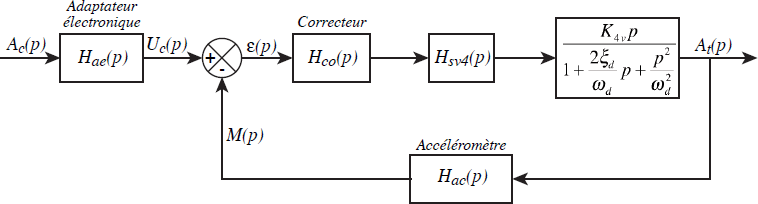
\includegraphics[width=0.7\linewidth]{fig_21}
\caption{Schéma-blocs simplifié du contrôle du mouvement de la table \label{fig_21}}
\end{figure}


Afin de satisfaire le critère de précision en poursuite du cahier des charges on place un premier correcteur
de type double intégrateur non unitaire de fonction de transfert : $H_{\text{CO}}(p)=\dfrac{K_{i2}}{p^2}$

La valeur de $K_{i2}$ est déterminée afin d’obtenir une pulsation à \SI{0}{dB} de la Fonction de Transfert en Boucle
Ouverte de $\SI{1000}{rad.s^{-1}}$.

\subparagraph{\label{q_41}}\textit{Donner la Fonction de Transfert en Boucle Ouverte de l’asservissement et préciser son mode
dominant.}
\ifprof
\begin{corrige} ~\\

\end{corrige}
\else
\fi

Le diagramme de Bode de cette Fonction de Transfert en Boucle Ouverte simplifiée est donné sur la
\autoref{fig_22}.

\begin{figure}[H]
\centering
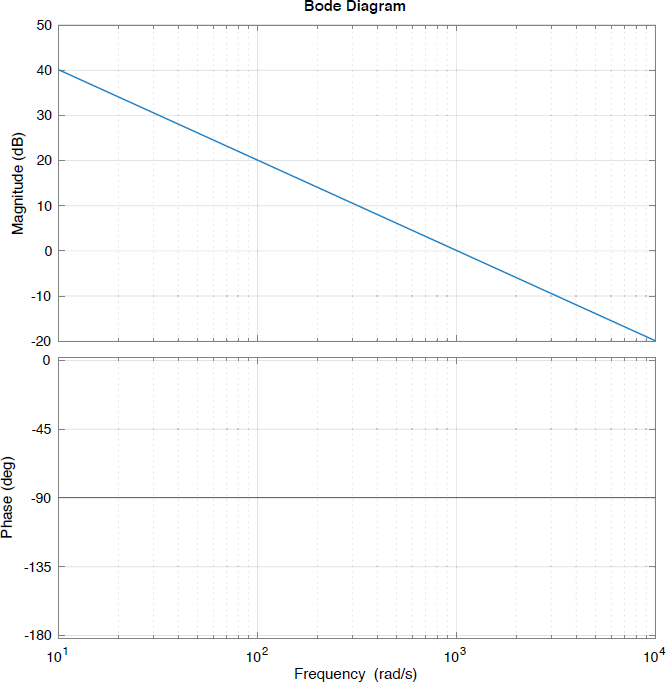
\includegraphics[width=0.7\linewidth]{fig_22}
\caption{Diagramme de Bode de la FTBO simplifiée \label{fig_22}}
\end{figure}


\subparagraph{\label{q_42}}\textit{Quels sont les critères du cahier des charges validés actuellement ?}
\ifprof
\begin{corrige} ~\\

\end{corrige}
\else
\fi

Un essai est réalisé sur le système. Une entrée en rampe d’accélération est imposée en entrée du système.
L’évolution temporelle de tension délivrée par l’accéléromètre est donnée sur la \autoref{fig_23}.

\subparagraph{\label{q_43}}\textit{Quel critère n’est pas vérifié sur le système réel ? En regardant attentivement le début de
la courbe de la \autoref{fig_19}, identifier le phénomène en cause et préciser la valeur de son
coefficient caractéristique. Préciser quels peuvent être les sous-systèmes pouvant provoquer
l’apparition de ce phénomène. Quel terme doit-on ajouter à la Fonction de Transfert en
Boucle Ouverte du système afin de prendre en compte ce phénomène.}
\ifprof
\begin{corrige} ~\\

\end{corrige}
\else
\fi

Afin de corriger l’effet de ce phénomène, on place un intégrateur supplémentaire de gain $K_{i3}$ :
$H_\text{CO}(p)=\dfrac{K_{i2}K_{i3}}{p^3}$.

\subparagraph{\label{q_44}}\textit{Préciser la valeur de $K_{i3}$ qui permet de retrouver la bande passante à \SI{1000}{rad.s^{-1}}.}
\ifprof
\begin{corrige} ~\\

\end{corrige}
\else
\fi

\begin{figure}[H]
\centering
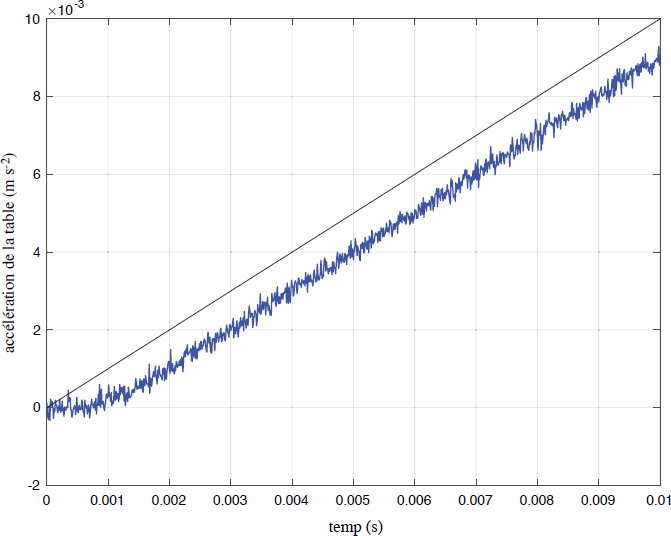
\includegraphics[width=0.6\linewidth]{fig_23}
\caption{Réponse à une rampe unitaire \label{fig_23}}
\end{figure}

On donne sur le Document Réponses le diagramme de Bode du gain de la FTBO ainsi corrigée.


\subparagraph{\label{q_45}}\textit{Déterminer la valeur de la phase pour les pulsations 10, 100, 1 000 et \SI{10 000}{rad.s^{-1}} et tracer
à main levée, mais avec soin, le diagramme de la phase.}
\ifprof
\begin{corrige} ~\\

\end{corrige}
\else
\fi

Afin de vérifier le critère sur la marge de phase du Cahier des Charges, on ajoute un correcteur à avance de
phase de fonction de transfert : $H_{\text{ap}}(p) = K_{\text{ap}}\dfrac{1+\tau_{\text{ap}}}{1+a_{\text{ap}}\tau_{\text{ap}}p}$ avec $a_{\text{ap}}<1$.

\subparagraph{\label{q_46}}\textit{À partir des documents donnés en annexes, déterminer les valeurs approximatives des paramètres $a_{\text{ap}}$, $\tau_{\text{ap}}$ et $K_{\text{ap}}$ qui permettent de satisfaire le critère de marge de phase du cahier
des charges tout en conservant une pulsation à \SI{0}{dB} de \SI{1 000}{rad.s^{-1}}.}
\ifprof
\begin{corrige} ~\\

\end{corrige}
\else
\fi

Le régulateur étant a priori optimisé, on réalise un essai de validation du comportement temporel de la
table. Le calculateur envoie un signal de consigne correspondant à une rampe de pente unitaire. L’accélération
de la table obtenue à partir de la mesure de l’accéléromètre est représentée sur la \autoref{fig_24}.

\begin{figure}[H]
\centering
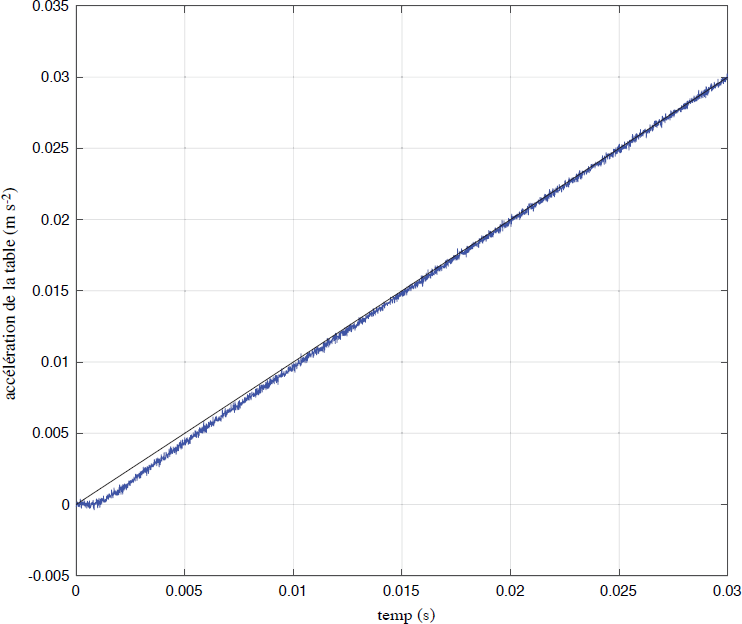
\includegraphics[width=0.5\linewidth]{fig_24}
\caption{Essai de validation \label{fig_24}}
\end{figure}

\subparagraph{\label{q_47}}\textit{Conclure quant au comportement observé.}
\ifprof
\begin{corrige} ~\\

\end{corrige}
\else
\fi

\section{Annexe A}
\subsection{Système du second ordre}

\begin{figure}[H]
\centering
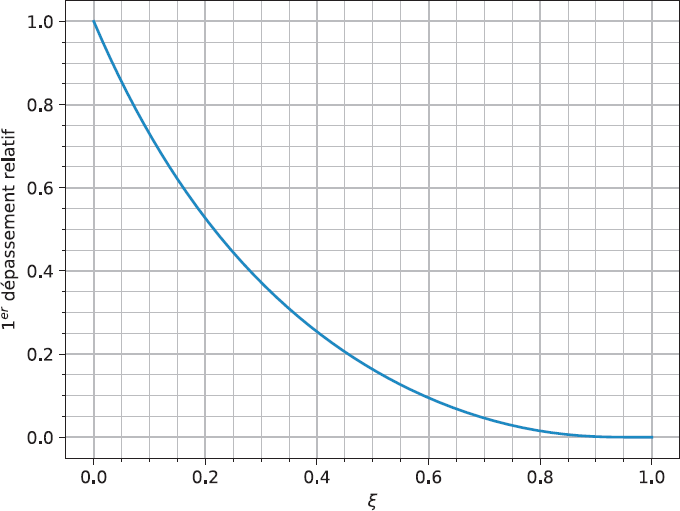
\includegraphics[width=.6\linewidth]{fig_25}
\caption{Graphe donnant le premier d´epassement relatif à la valeur finale de la réponse
indicielle d’une FT du second ordre en fonction du coefficient d’amortissement
 \label{fig_25}}
\end{figure}

\subsection{Correcteur à avance de phase}


\begin{figure}[H]
\centering
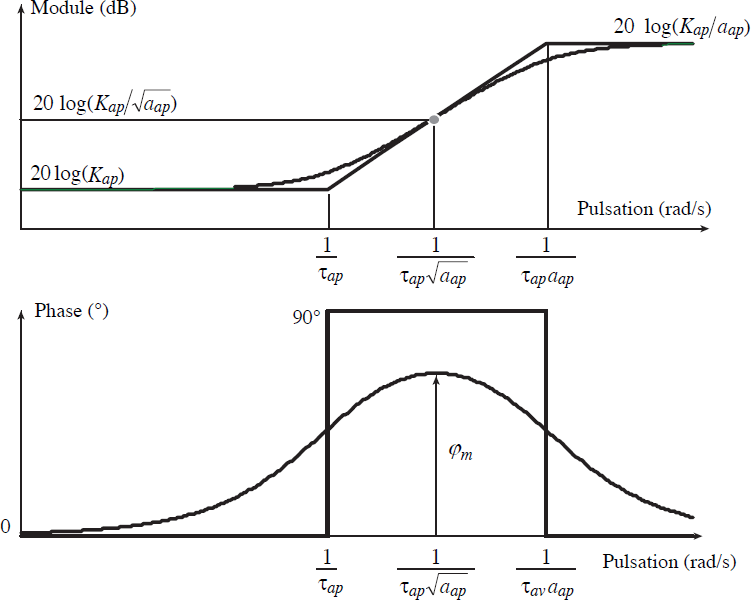
\includegraphics[width=.6\linewidth]{fig_26}
\caption{Diagramme de Bode d’un correcteur à avance de phase  \label{fig_26}}
\end{figure}

\begin{figure}[H]
\centering
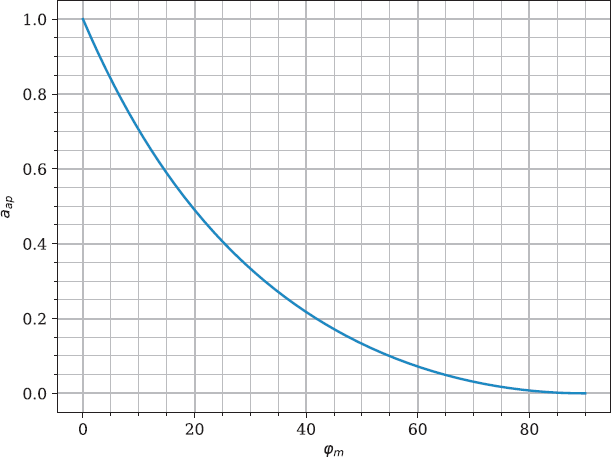
\includegraphics[width=.6\linewidth]{fig_27}
\caption{Graphe donnant $a_{ap}$ en fonction de $\varphi_m$ \label{fig_27}}
\end{figure}


\section{Annexe B}
\begin{figure}[H]
\centering
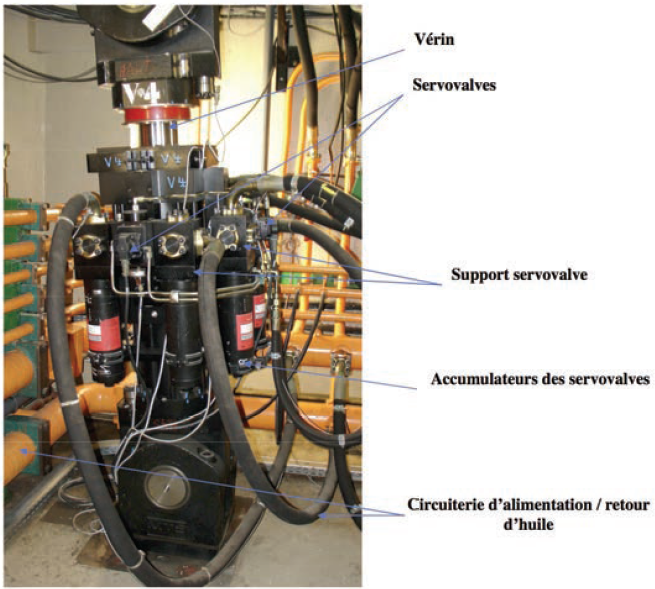
\includegraphics[width=.8\linewidth]{ann_b_01}
\end{figure}
\begin{figure}[H]
\centering
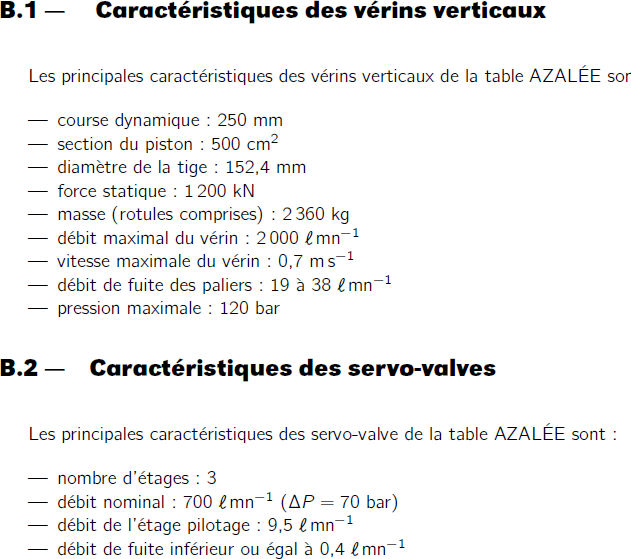
\includegraphics[width=.8\linewidth]{ann_b_02}
\end{figure}
\newpage





\textbf{Questions \ref{q_23} et \ref{q_24}}

\begin{figure}[H]
\centering
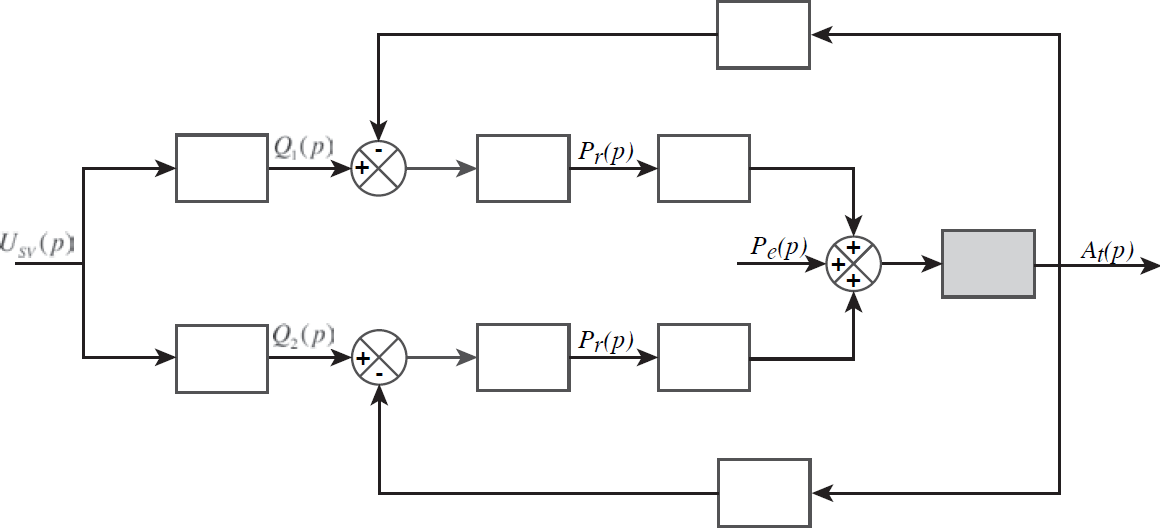
\includegraphics[width=.8\linewidth]{q_23}
\end{figure}




\textbf{Questions \ref{q_31} et \ref{q_33}}

\begin{figure}[H]
\centering
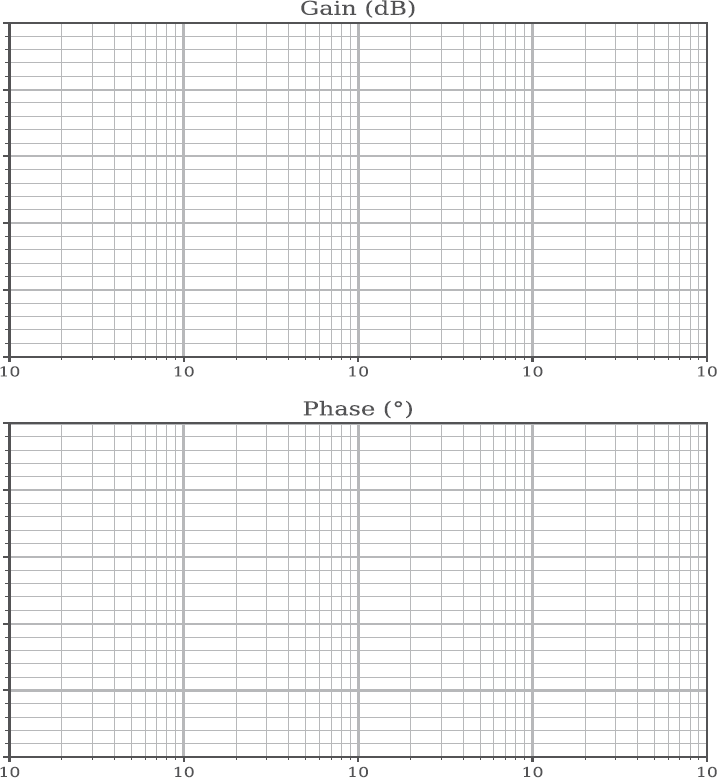
\includegraphics[width=.8\linewidth]{q_31}
\end{figure}

\newpage

\textbf{Question \ref{q_45} }
\begin{figure}[H]
\centering
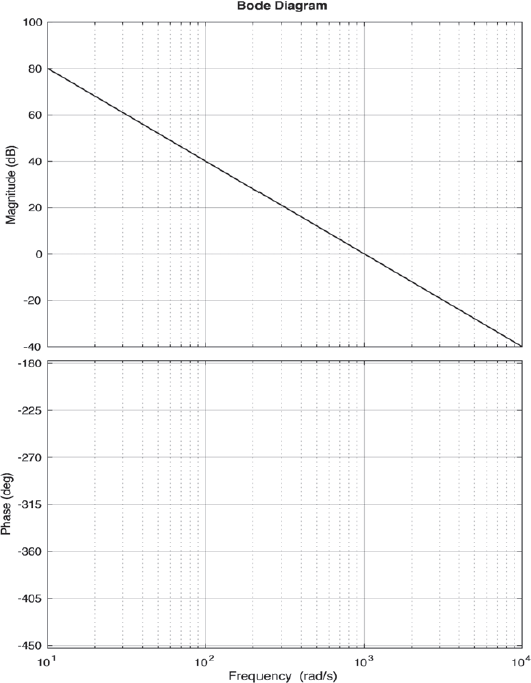
\includegraphics[width=.8\linewidth]{q_45}
\end{figure}


\end{document}



